%%%%%%%%%%%%%%%%%%%% author.tex %%%%%%%%%%%%%%%%%%%%%%%%%%%%%%%%%%%
%
% sample root file for your "contribution" to a contributed volume
%
% Use this file as a template for your own input.
%
%%%%%%%%%%%%%%%% Springer %%%%%%%%%%%%%%%%%%%%%%%%%%%%%%%%%%


% RECOMMENDED %%%%%%%%%%%%%%%%%%%%%%%%%%%%%%%%%%%%%%%%%%%%%%%%%%%
\RequirePackage{rotating}
\documentclass[graybox]{svmult}

% choose options for [] as required from the list
% in the Reference Guide

\usepackage{mathptmx}       % selects Times Roman as basic font
\usepackage{helvet}         % selects Helvetica as sans-serif font
\usepackage{courier}        % selects Courier as typewriter font
\usepackage{type1cm}        % activate if the above 3 fonts are
                            % not available on your system
%
\usepackage{makeidx}         % allows index generation
\usepackage{graphicx}        % standard LaTeX graphics tool
                             % when including figure files
\usepackage{multicol}        % used for the two-column index
\usepackage[bottom]{footmisc}% places footnotes at page bottom



% see the list of further useful packages
% in the Reference Guide

%%%%%%%%%%% New packages and commands %%%%%%%%%%%%%%%%%%%%%%%%%%%%%%%%%%%%%%%%%%%%%%%%%%%%%

\usepackage{times,appendix}
\usepackage{epsfig}
\usepackage{graphicx}
\usepackage{color,url}
%\usepackage[sort&compress]{natbib}
%\usepackage{hyperref}
\newcommand{\theHalgorithm}{\arabic{algorithm}}
\usepackage{rotating,lscape,pdflscape}
\usepackage{wrapfig}
\usepackage{sidecap}
\sidecaptionvpos{figure}{c}

%%% load AMS-Latex Package
%\usepackage{amsmath,amsfonts}
%\usepackage{amsthm,amssymb,amsopn}
%\usepackage{amsthm,amssymb,amsopn}
\usepackage{amsmath,amssymb,amsopn}
\usepackage{bm} % bold symbol
\usepackage{booktabs, tabu}

% define fonts
\newcommand{\vct}[1]{\boldsymbol{#1}} % vector
\newcommand{\mat}[1]{\boldsymbol{#1}} % matrix

%%%% Special math symbols
\newcommand{\field}[1]{\mathbb{#1}}
\newcommand{\R}{\field{R}} % real domain
\newcommand{\C}{\field{C}} % complex domain
\newcommand{\F}{\field{F}} % functional domain
%\newcommand{\T}{^{\top}\!\!} % transpose
\newcommand{\T}{^{\textrm T}} % transpose
\newcommand{\TN}{^{-\textrm T}} % transpose


%%% define constant
\newcommand{\cst}[1]{\mathsf{#1}}

%% operator in linear algebra, functional analysis
\newcommand{\inner}[2]{#1\cdot #2}
\newcommand{\norm}[1]{\|#1\|}
\newcommand{\twonorm}[1]{\|#1\|_2^2}
% operator in functios, maps such as M: domain1 --> domain 2
\newcommand{\Map}[1]{\mathcal{#1}}

% operator in probability: expectation, covariance,
\newcommand{\ProbOpr}[1]{\mathbb{#1}}
% independence
\newcommand\independent{\protect\mathpalette{\protect\independenT}{\perp}}
\def\independenT#1#2{\mathrel{\rlap{$#1#2$}\mkern2mu{#1#2}}}
% conditional independence
\newcommand{\cind}[3]{{#1} \independent{#2}\,|\,#3}
% conditional expectation
\newcommand{\cndexp}[2]{\ProbOpr{E}\,[ #1\,|\,#2\,]}

% operator in optimization
\DeclareMathOperator{\argmax}{arg\,max}
\DeclareMathOperator{\argmin}{arg\,min}
\newcommand{\todo}[1]{{\color{red}#1}}


% environment
\newtheorem{thm}{Theorem}
%\newtheorem{lemma}{Lemma}

\newcommand{\eat}[1]{}

% \usepackage{mathptmx}      % use Times fonts if available on your TeX system
% Insert the name of "your journal" with
% \journalname{myjournal}

%%%%%%% ANNOTATING COMMAND %%%%%%%%%%%%%

\newcommand{\source}{{S}}
\newcommand{\target}{{T}}
\newcommand{\landmark}{\mathcal{L}^q}
\newcommand{\mkltrain}{\mathcal{D}_{\textsc{train}}}
\newcommand{\mkltest}{\mathcal{D}_{\textsc{dev}}}
\newcommand{\src}{\mathcal{D}_{S}}
\newcommand{\tgt}{\mathcal{D}_{T}}
\newcommand{\ltarget}{\mathcal{D}_\mathcal{L}}
\newcommand{\utarget}{\mathcal{D}_\mathcal{U}}
\newcommand{\srcbase}{\mat{P}_{S}}
\newcommand{\tgtbase}{\mat{P}_{T}}
\newcommand{\stbase}{\mat{P}_{{S}+{T}}}
\newcommand{\srcpca}{\textbf{PCA}_{S}}
\newcommand{\srcpls}{\textbf{PLS}_{S}}
\newcommand{\tgtpca}{\textbf{PCA}_{T}}
\newcommand{\stpca}{\textbf{PCA}_{{S}+{T}}}
\newcommand{\stpls}{\textbf{PLS}_{{S}+{T}}}
\newcommand{\srccomp}{\mat{R}_{S}}
\newcommand{\kernel}{\mat{G}}

\newcommand{\blue}[1]{\textcolor{blue}{#1}}
\newcommand{\red}[1]{\textcolor{red}{#1}}


\newcommand{\OrigFeat}{\textsc{no adapt}}
\newcommand{\PCAs}{\textsc{pca}$_{{S}}$}
\newcommand{\PCAt}{\textsc{pca}$_{{T}}$}
\newcommand{\PCAst}{\textsc{pca}$_{{S}+{T}}$}
\newcommand{\PLSs}{\textsc{pls}$_{{S}}$}
\newcommand{\PLSt}{\textsc{pls}$_{{T}}$}
\newcommand{\PLSst}{\textsc{pls}$_{{S}+{T}}$}
%\newcommand{\discSample}{{{Discrete Sample}}}
\newcommand{\ICCV}{\textsc{gfs}}
\newcommand{\ECCV}{\textsc{metric}}
\newcommand{\GEO}{\textsc{gfk}(\PCAs, \PCAt)}
\newcommand{\plsGEO}{\textsc{gfk}(\PLSs, \PCAt)}
\newcommand{\plsGEOpls}{\textsc{gfk}(\PLSs, \PLSt)}
\newcommand{\GFK}{\textsc{gfk}}
\newcommand{\caltech}{{\textsc{caltech}}}
\newcommand{\amazon}{{\textsc{amazon}}}
\newcommand{\dslr}{{\textsc{dslr}}}
\newcommand{\webcam}{{\textsc{webcam}}}
\newcommand{\bline}{{\textsc{baseline}}}
\newcommand{\ours}{{\textsc{landmark}}}

\newcommand{\fix}{\marginpar{FIX}}
\newcommand{\new}{\marginpar{NEW}}
\newcommand{\ie}{\emph{i.e.}}
\newcommand{\etal}{\emph{et al.}}

\newcommand{\FS}[1]{{\color{red}#1}}
%\newcommand{\FS}[1]{}
\newcommand{\KG}[1]{{\color{blue} KG: #1}}
%\newcommand{\KG}[1]{}
\newcommand{\BG}[1]{{\color{magenta} #1}}
%\newcommand{\BG}[1]{}

% Bib aliases
\makeatletter
\def\@citex[#1]#2{\leavevmode
  \let\@citea\@empty
  \@cite{\@for\@citeb:=#2\do
    {\@citea\def\@citea{,\penalty\@m\ }%
\edef\magic##1{\let##1\expandafter\noexpand\csname bibalias@\@citeb\endcsname}%
\magic\tmp \ifx\tmp\relax\else \let\@citeb\tmp\fi
     \edef\@citeb{\expandafter\@firstofone\@citeb\@empty}%
     \if@filesw\immediate\write\@auxout{\string\citation{\@citeb}}\fi
     \@ifundefined{b@\@citeb}{\hbox{\reset@font\bfseries ?}%
       \G@refundefinedtrue
       \@latex@warning
         {Citation `\@citeb' on page \thepage \space undefined}}%
       {\@cite@ofmt{\csname b@\@citeb\endcsname}}}}{#1}}
\def\bibalias#1#2{\expandafter\def\csname bibalias@#1\endcsname{#2}}
\makeatother

\bibalias{shimodaira00shift}{ShimodairaJSPI00Improving}
\bibalias{daume06domain}{DaumeJAIR06Domain}
\bibalias{pan2009survey}{PanTKDE10Survey}
\bibalias{gretton09kmm}{GrettonBC09Covariate}
\bibalias{gopalan2011domain}{GopalanICCV11Domain}
\bibalias{gong12gfk}{GongCVPR12Geodesic}
\bibalias{chen11cotrain}{ChenNIPS11Cotraining}
\bibalias{daume10co}{DaumeNIPS10co}
\bibalias{bergamo09weak}{BergamoNIPS10Exploiting}
\bibalias{saenko2010adapting}{SaenkoECCV10Adapting}
\bibalias{daume07easy}{DaumeX09Frustratingly}
\bibalias{blitzer11domain}{BlitzerAISTATS11Domain}
\bibalias{bendavid07domain}{BendavidNIPS07Analysis}
\bibalias{BenDavid10Adaptation}{BenDavidML10A}
\bibalias{tca}{PanTNN11Domain}
\bibalias{mansour09domain}{MansourCOLT09Domain}
\bibalias{mansour09multiple}{MansourUAI09multiple}
\bibalias{lanckriet04kernel}{LanckrietJMLR04kernel}
\bibalias{mkl_obj}{VedaldiICCV09multiple}
\bibalias{ham2004kernel}{HamICML04kernel}
\bibalias{roweis2000nonlinear}{RoweisSCI00nonlinear}
\bibalias{weinberger2006unsupervised}{WeinbergerIJCV06unsupervised}
\bibalias{hamm2008grassmann}{HammICML08grassmann}
\bibalias{gong13landmark}{GongICML13Connecting}
\bibalias{gretton2006kernel}{GrettonNIPS06kernel}
\bibalias{Caltech256}{Griffin07Caltech}
\bibalias{kulisyou}{KulisCVPR11What}
\bibalias{bay2006surf}{BayECCV06Surf}
\bibalias{PLS}{Hastie09Elements}
\bibalias{huang07correcting}{HuangNIPS07Correcting}
\bibalias{ando05}{AndoJMLR05framework}
\bibalias{li2012discriminative}{LiCVPR12discriminative}
\bibalias{zheng2012grassmann}{ZhengCVPR12Grassmann}
\bibalias{bruzzone2010domain}{BruzzonePAMI10Domain}
\bibalias{shi2012}{ShiICML12Informationtheoretical}
\bibalias{dam}{DuanTNNLS12Domain}
\bibalias{dredze08multi}{DredzeEMNLP08multi}
\bibalias{our2013reshape}{GongNIPS13Reshaping}
\bibalias{gopalan2013learning}{GopalanCVPR13learning}
\bibalias{bergamo09weak}{BergamoNIPS10Exploiting}
\bibalias{bergamo09weak}{BergamoNIPS10Exploiting}
\bibalias{bergamo09weak}{BergamoNIPS10Exploiting}
\bibalias{bergamo09weak}{BergamoNIPS10Exploiting}
\bibalias{bergamo09weak}{BergamoNIPS10Exploiting}
\bibalias{bergamo09weak}{BergamoNIPS10Exploiting}
\bibalias{bergamo09weak}{BergamoNIPS10Exploiting}





%%%%%%%%%%%%%%%%%%%%%%%%%%%%%%%%%%%%%%%%%%%%%%%%%%%%%%%%%%%%%%%%%%%%%%%%%%%%%%%%%%%%%%%%





\makeindex             % used for the subject index
                       % please use the style svind.ist with
                       % your makeindex program

%%%%%%%%%%%%%%%%%%%%%%%%%%%%%%%%%%%%%%%%%%%%%%%%%%%%%%%%%%%%%%%%%%%%%%%%%%%%%%%%%%%%%%%%%

\begin{document}
\setlength{\belowdisplayskip}{5pt} \setlength{\belowdisplayshortskip}{2pt}
\setlength{\abovedisplayskip}{5pt} \setlength{\abovedisplayshortskip}{2pt}

\title*{Geodesic Flow Kernel and Landmarks: 
Kernel Methods for Unsupervised Domain Adaptation}
\titlerunning{Kernel Methods for Unsupervised Domain Adaptation}
% Use \titlerunning{Short Title} for an abbreviated version of
% your contribution title if the original one is too long
\author{Boqing Gong, Kristen Grauman, and Fei Sha}
% Use \authorrunning{Short Title} for an abbreviated version of
% your contribution title if the original one is too long
\institute{Boqing Gong \at University of Central Florida, Orlando, FL, 32816, \email{boqinggong@gmail.com}
\and Kristen Grauman \at  University of Texas at Austin, TX, 78712, \email{grauman@cs.utexas.edu}
\and Fei Sha \at University of California at Los Angeles, CA, 90095, \email{feisha.work@gmail.com}}
%
% Use the package "url.sty" to avoid
% problems with special characters
% used in your e-mail or web address
%
\maketitle

\abstract{Domain adaptation aims to correct the mismatch in statistical properties between the source domain on which a classifier is trained and the target domain to which the classifier is to be applied. In this chapter, we address the challenging scenario of \emph{unsupervised domain adaptation}, where the target domain does not provide any annotated data to assist in adapting the classifier. Our strategy is to learn robust features which are resilient to the mismatch across domains and then  use them  to construct classifiers that will perform well on the target domain. 
\newline \indent
To this end, we propose novel kernel learning approaches to inferring such features for adaptation.  Concretely, we explore two closely related directions. In the first direction, we propose \emph{unsupervised learning} of a geodesic flow kernel (GFK). GFK summarizes the inner products in an infinite sequence of feature subspaces that smoothly interpolates between the source and target domains. In the second direction, we propose \emph{supervised learning} of a kernel that discriminatively combines  multiple base GFKs. Those base kernels model the source and the target domains at fine-grained granularities. In particular, each base kernel pivots on a different set of landmarks -- the most useful data instances that reveal the similarity between the source and the target domains, thus bridging them to achieve adaptation. 
\newline \indent
Our approaches are computationally convenient and are capable of learning features/kernels and classifiers discriminatively without demanding labeled data from the target domain.  In extensive empirical studies on standard benchmark object recognition datasets, our approaches outperform a variety of competing methods.}



%%%%%%% MAIN BODY %%%%%%%%%%%%%


\section{Introduction}
\begin{figure*}[t]
\centering
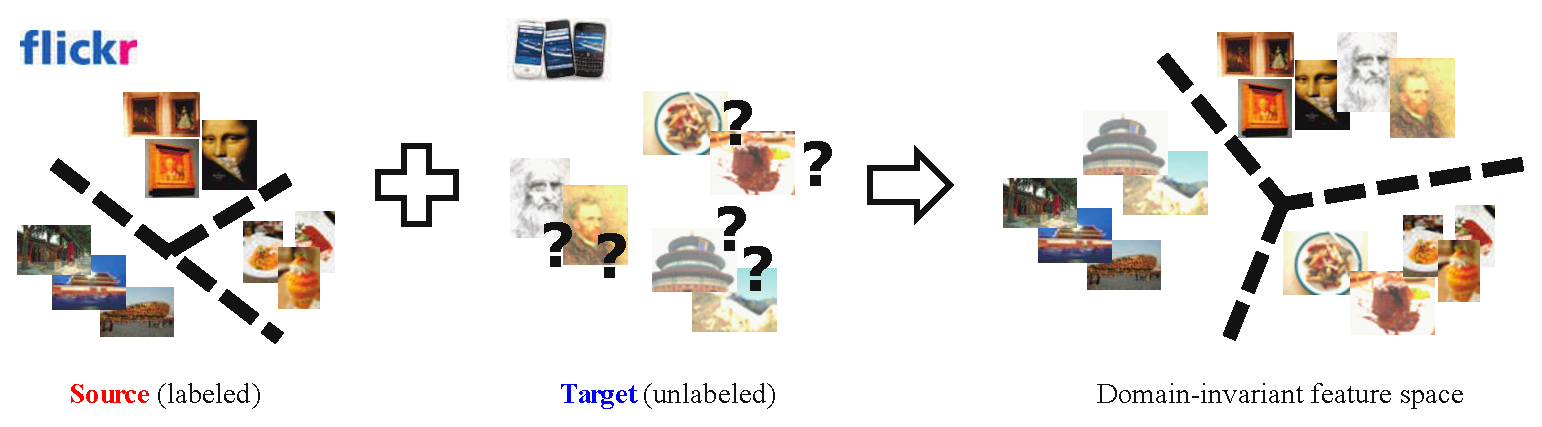
\includegraphics[width=0.92\columnwidth]{fig/fImageConcept_3.eps}
\caption{An illustrative example of {\bf unsupervised domain adaptation}. The goal is to classify unlabeled data from the \blue{target} domain that has different characteristics from the \red{source} domain where annotated data are provided. The central idea behind our approaches is to use the data from both domains to infer a domain-invariant feature/kernel space such that, in this space, the classifier learned using the labels of the source domain will likely work well on the target domain.}
\label{fConceptUDA}
\end{figure*}

Statistical machine learning algorithms often rely on the assumption that data used for training and testing are drawn from the same distribution. However, the validity of this assumption is frequently challenged in real-world applications. Figure~\ref{fConceptUDA} gives an illustrative example. Imagine that we are to deploy an APP to recognize images captured by mobile phone cameras. Instead of demanding that users provide labels to our learning algorithms, can we train classifiers with existing tagged Flickr images, and hope the classifiers will still work well on mobile camera test images? Our intuition says no. We suspect that the strong distinction between the Flickr images and the typical mobile phone images will cripple the classifiers.

Indeed, a stream of studies has shown that when the classifiers for object recognition are evaluated outside of their training datasets, the performance degrades significantly~\cite{TorralbaCVPR11Unbiased,DollarCVPR09Pedestrian,PerronninCVPR10Largescale}.  The culprit is clear: the visual appearance  of even the same object varies across different datasets as a result of many factors, such as imaging devices, photographers' preferences, and background. These idiosyncrasies often cause a substantial mismatch between the training and testing data. In addition to object recognition, the mismatch is also abundant in other computer vision tasks~\cite{DuanCVPR09Domain,WangCVPR2011automatic,JainCVPR10online,DuanPAMI12Visual}, speech recognition~\cite{LeggetterCSL95Maximum}, and text analysis~\cite{BlitzerACL07domain,BlitzerEMNLP06Domain}. 






In all these pattern recognition tasks, there is a common theme. There are  two distinct types of datasets: one from a \textbf{source} domain and the other from a \textbf{target} domain. The source domain contains a large amount of labeled data such that a classifier can be reliably built. The target domain refers broadly to a related dataset that has different characteristics compared to the source domain.  In other words, the underlying distributions of the datasets are different. Note that we assume the set of possible labels remains the same across domains.



%Thus, the main objective is to \emph{adapt} classifiers trained on the source domain to the target domain to attain good performance there.

\subparagraph{How to build classifiers that are robust to the mismatched distributions?}
Techniques for addressing this challenge have been  investigated under the names of domain adaptation, covariate shift, or  transfer learning~\cite{shimodaira00shift,daume06domain,pan2009survey,gretton09kmm}. When there is no labeled data from the target domain to help learning, the problem, illustrated in Fig.~\ref{fConceptUDA},  is called \textbf{{unsupervised domain adaptation}}~\cite{BlitzerACL07domain,BlitzerEMNLP06Domain,gopalan2011domain,gong12gfk,chen11cotrain}. When some labeled  data from the target domain is accessible (but insufficient for constructing a good classifier), the problem is similar to semi-supervised learning and is named semi-supervised domain adaptation \cite{daume10co,bergamo09weak,saenko2010adapting}. In either case, how to effectively leverage \emph{unlabeled} target data is key to domain adaptation.


%We focus on unsupervised domain adaptation in this chapter as it is highly desirable in real-world applications. It taxes users minimally, as the recognition system adapts automatically. While appealing, unsupervised domain adaptation is especially challenging. For example, the common practice of discriminative training is generally not applicable. Without labels, it is not even clear how to define the right discriminative loss on the target domain! Similarly, it is also difficult to perform model selection.% (e.g., tuning regularization coefficients).

%We focus on overcoming those challenges.  Our core idea is to model how the source and target are related in order to enable unsupervised domain adaptation. Our effort centers around the notion of learning kernel functions as a way to infer robust features that are resilient (``invariant") to the mismatch between domains.

Discovering domain-invariant feature spaces that enable the adaptation of classifiers or regressors has been an extensively studied paradigm~\cite{bendavid07domain,BlitzerEMNLP06Domain,BlitzerACL07domain,daume07easy,tca}. The feature representation can be derived using auxiliary tasks that predict ``pivot features''~\cite{ando05,BlitzerEMNLP06Domain}, augmenting the feature space~\cite{daume07easy,daume10co,li2012discriminative,gopalan2013learning}, co-training with multi-view representations~\cite{chen11cotrain}, or matching probabilistic distributions~\cite{tca}. In a such space, the source and target domains have the same (or similar) marginal distributions over the input data, and the posterior distributions of the labels are often assumed to be the same across domains too. Hence, a conventional classifier trained on the labeled source would  likely  perform  well on the target. Some theoretical analyses show that the generalization capability of the classifier on the target is indeed positively correlated with the domain-invariance, measured by different metrics, of the learned feature spaces~\cite{BenDavid10Adaptation,mansour09domain,mansour09multiple}.

Many existing feature learning methods in domain adaptation, however, are not directly applicable to {\em visual recognition}. For instance, the bag-of-words representations in natural language process often contain semantic and discriminative ``pivot'' features that transfer across domains~\cite{daume07easy,BlitzerEMNLP06Domain,BlitzerACL07domain,chen11cotrain}; to determine the sentiments (\textsc{positive} versus \textsc{negative}) of consumers' product reviews, words like ``do not buy'' transcend product categories. In computer vision tasks, this intuition no longer holds. Often, no single feature  is discriminative enough for visual recognition tasks.

\subparagraph{How can we infer an invariant feature space from \emph{visual} data?} 

We therefore propose novel approaches to unsupervised domain adaptation, with applications to visual recognition in mind. We focus on unsupervised domain adaptation as it is highly desirable in real-world applications. It taxes users minimally by automatically adapting the visual recognition systems. While appealing, unsupervised domain adaptation is especially challenging. For example, the common practice of discriminative training is generally not applicable. Without labels, it is not even clear how to define the right discriminative loss on the target domain! Similarly, it is also difficult to perform model selection.% (e.g., tuning regularization coefficients).

We overcome those challenges by leveraging the conceptual connection between features and kernels, in order to better relate the source and target domains. Instead of explicitly defining which features are domain-invariant, we discover them \emph{implicitly} by learning kernel functions that compute the inner products between data points in a (transformed) feature space. Thus, inferring domain-invariant feature spaces is equivalent to learning kernel functions that ``host'' those features.

Learning kernels has been employed in a variety of problems in computer vision and machine learning~\cite{lanckriet04kernel,mkl_obj,ham2004kernel,roweis2000nonlinear,weinberger2006unsupervised}. As our ultimate goal is to build a classifier that performs well on the target, the framework of discriminatively combining multiple kernels is especially appealing~\cite{lanckriet04kernel}. To this end, we need address two crucial and interdependent questions: what to use as base kernels, and how to discriminatively combine them when there is no labeled data from the target domain?  

Our solution rests on two novel modeling considerations in a seamless fashion. The first  leads to the development of the {\bf geodesic flow kernel (GFK)}~\cite{GongCVPR12Geodesic}, and is based on the idea of intermediate feature spaces. Analogous to unsupervised manifold learning of kernels, GFK exploits the structures of low-dimensional subspaces in visual data. It measures the data pairwise similarities that are insensitive to variations in domains. In particular, it results from aggregating the inner products computed within a sequence of infinite subspaces interpolating between the source and target domains. While each subspace may idiosyncratically favor the source or the target domain, the aggregation smooths out the idiosyncrasies. Consequently, when used in a nearest neighbor classifier as a similarity measure, GFK outperforms many competing methods for domain adaptation. The kernel function can be computed without requiring any labels from the target domain and can be plugged into any kernel-based classifier. We present the details in section~\ref{sGFK}. 

Our second modeling consideration aims to further improve GFK's discriminative power, centering around the notion of \textbf{landmarks}~\cite{GongICML13Connecting}. Concretely, we exploit the insight that \emph{not all instances from the source domain are created equally in terms of adaptability}~\cite{GongICML13Connecting}.  Existing research in modeling the discrepancy between domains has been limited to macroscopically examining their distribution similarity by tuning to statistical properties of the samples as a whole --- when comparing (marginal) distributions to derive features, all the samples are used. This notion  is stringent, as it requires all discrepancies to  be accounted for and forces learning inefficiently (or even erroneously) from ``hard'' cases that might be just outliers to the target domains (cf.\ examples in Fig.~\ref{fLandmark}).

In contrast, we examine distribution similarity microscopically at the instance level.  Our approach automatically plucks out and exploits the most desirable {\bf ``landmark"} instances from the source domain. The landmarks bridge the source and the target domains at a fine granularity; they are labeled instances from the source domain that are distributed similarly to the target domain. As a result, the labels of the landmarks serve as a good proxy for us to approximate the discrimintive loss on the target domain. We show how to use those landmarks to construct multiple domain-invariant features (i.e., multiple GFKs) and how those kernels can be discriminatively combined to learn a new domain-invariant feature space such that the adapted classifier performs the best on the target domain  (cf.\ section~\ref{sLandmark}).


We conduct extensive empirical studies to validate our approaches on the task of visual object recognition, where we train classifiers on one dataset and then apply them to others (section~\ref{sExp}). Section~\ref{sConclusion} concludes this chapter. 


\section{Learning kernels for unsupervised domain adaptation}
This section presents our kernel approach to unsupervised domain adaptation. We first derive the base geodesic flow kernels that entail domain-invariant features and infinite subspaces between the source and target domains, and then develop the landmark based algorithm to combine the base kernels with approximated discriminative loss of the target. Our emphasis on the kernel learning aspect sheds light on future research. We believe the core paradigm of learning invariant features for domain adaptation can be further advanced by a broader set of kernel  techniques. 


\eat{
{\bf Contributions.} 
Our main contributions lie in developing new kernel learning methods for unsupervised domain adaptation and validating their effectiveness in object recognition. Our emphasis on the kernel learning aspect not only provides a natural connection between our two approaches, GFK~\cite{GongCVPR12Geodesic} and the landmark-based domain adaptation~\cite{GongICML13Connecting}, but also sheds light on future research directions. Specifically, we believe the core paradigm of learning invariant feature spaces can be further advanced by a broader set of kernel learning techniques.  %In addition, we present significantly more details on our empirical studies and an improved exposition of key ideas and algorithms. 


In section~\ref{sGFK}, we derive our \textbf{geodesic flow kernel (GFK)} --- a kernel function that exploits intrinsic low-dimensional subspaces in visual data and measures similarity using those subspaces. The kernel function can be computed without requiring any labels from the target domain and can be plugged into any kernel-based classifier. Furthermore, using the kernel avoids cross-validation of hyperparameters.

In section~\ref{sLandmark}, we develop an approach that further improves GFK's discriminative power. The  approach centers around the notion of \textbf{landmarks}. Landmarks reveal domain similarity at a fine granularity; they are defined as a subset of labeled instances from the source domain that are distributed similarly to the target domain. Thus, they are expected to function as a conduit \emph{connecting} the source and target domains to facilitate adaptation. We show how to use those landmarks to construct multiple domain-invariant features (i.e., multiple GFKs) and how those kernels can be discriminatively combined to learn a new domain-invariant feature space such that the adapted classifier performs the best on the target domain.

}

% !TEX root = da.tex

\subsection{The base geodesic flow kernel (GFK)}  \label{sGFK}


\begin{figure*}[t]
\centering
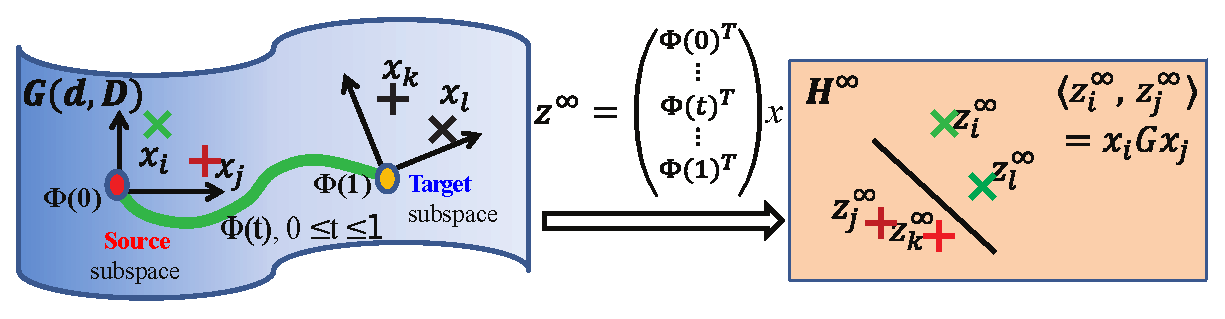
\includegraphics[width=0.9\columnwidth]{fig/fConcept4}
\caption{Main idea of our geodesic flow kernel (GFK). The source and target domains are embedded in a Grassmann manifold, which is a collection of all $d$-dimensional subspaces of $\R^\cst{D}$. We connect the two subspaces of the two domains by a continuous geodesic flow $\mat{\Phi(t)}$. After projecting a data point $\vct{x}$ to this flow, we arrive at an infinitely dimensional feature vector $\vct{z}^\infty\in\mathcal{H}^\infty$ which encapsulates incremental changes from the source subspace to the target subspace. As a result, the inner product between two such vectors ``averages out'' the domains' idiosyncrasies and can be analytically computed in a closed form. (best viewed in color)}
\label{fConceptGFK}
\end{figure*}

\eat{
\subsection{Main idea} \label{sGFK-main}
Our approach  follows broadly the theme of identifying the \emph{shared representation} between different domains~\cite{bendavid07domain}. Intuitively, we seek a feature space such that when data points are projected into this space, the source domain is similar to the target domain. How to define and quantify shared characteristics entails careful examination of our intuition on what type of representation facilitates adaptation. For example, in the part-of-speech (POS) task of tagging words into different syntactic categories \cite{BlitzerEMNLP06Domain}, the idea is to extract shared patterns from  auxiliary classification tasks that predict ``pivot features'', frequent words which are themselves discriminative in both domains.  While sensible for language processing tasks, typical histogram based features of low-level visual descriptors do not have the benefits of pivot ``visual words'' --- in general, no single feature dimension from a particular histogram bin is discriminative enough to differentiate visual categories.

On the other hand, many visual data {are} assumed to lie in low-dimensional subspaces.  Given data from two domains, \emph{how can we exploit the subspaces in these datasets, which can be telltale cues in revealing the underlying difference and commonness between the domains?}
}

GFKs serve as the basis for the second stage of our approach --- using landmarks to discriminatively combine multiple GFKs for classifying the target data. Our main idea behind GFK is to {\em implicitly} construct  a feature space that aggregates information on the source domain $ \src$, the target $\tgt$, and ``phantom'' domains interpolating between those two. In particular, the phantom domains represent incremental changes in the geometric and statistical properties between the two domains.

While each of the domains is represented with a subspace, the inner products in $\mathcal{H}^\infty$ are defined to integrate over an infinite number of such subspaces. Intuitively, this integration averages out domain-specific idiosyncrasies and computes similarity measures that are insensitive to domain mismatch. Equivalently, the inner products give rise to a kernel function that defines the kernel mapping from the original feature space to a domain-invariant feature space. Fig.~\ref{fConceptGFK} sketches the main idea.

In the following, we start by reviewing some basic notions of Grassmann manifolds. The subspaces of the source and target domains are represented as two points on one such manifold.  Furthermore, the phantom domains correspond to the points on the geodesic path connecting those two points. 

\subsubsection{Modeling domains on Grassmann manifold}
In statistical modeling, we often assume data can be embedded in a
low-dimensional linear subspace. For example, principal component
analysis (PCA) identifies the subspace where the variances of the
embedded data are maximized. It is convenient to refer to a subspace with its  basis $\mat{P}\in
\R^{\cst{D}\times \cst{d}}$, where $\cst{D}$ and $\cst{d}$ are the dimensions of the data and subspace, respectively. \eat{For
PCA, the basis is then the top $\cst{d}$ eigenvectors of the data's
covariance matrix.}   The collection of all $\cst{d}$-dimensional
subspaces form the Grassmannian $\mathbb{G}(\cst{d},\cst{D})$, a
smooth Riemannian manifold on which we can define  geometric, differential, and probabilistic structures.

As an intuitive example of how manifolds can help us tackle domain adaptation, imagine that we compute the subspaces of the datasets for the $ \src$ and $\tgt$ domains and map them to two points on a Grassmannian.  Intuitively, if these two points are close by, then the two domains could be similar in the distribution of their data. Thus, a source $\src$-trained classifier is likely to work well on the target $\tgt$.

However, \emph{what if these two domains are far apart on the manifold?} For example, suppose two datasets of car images with large differences in poses are placed far apart on the manifold.
We aim to use intermediate subspaces to learn domain-invariant features for adaptation.
Specifically, the intermediate subspaces would capture statistics of car images under poses interpolated between the source and the target domains. Being informed of all these different subspaces from the same category, the learning algorithms might be able to extract features that are less sensitive to variations in pose.
To this end, we will use the geodesic flow path to connect the two domains, where every point on this flow path is an intermediate subspace.


\subsubsection{Defining the geodesic flow kernel (GFK)}
\label{sGFK-detail}
Our approach consists of the following steps: i) determine the optimal dimensionality of the subspaces to embed domains; ii) construct the geodesic flow; iii) compute the geodesic flow kernel; iv) use the kernel to construct a classifier with the labeled data of the source domain. We defer describing step i) to the next section and focus on steps ii) and iii). For step ii), we state only the main computational steps; the detailed derivation can be found in \cite{gopalan2011domain} and references therein. Step iv) is omitted for brevity, as it is the same as constructing any other kernel-based classifiers.

{\bf Construct geodesic flow.}  Let $\srcbase, \tgtbase \in \R^{\cst{D}\times\cst{d}}$ denote the two sets of basis of the subspaces for the source and target domains, respectively. Let $\srccomp \in \R^{\cst{D}\times (\cst{D-d})}$ denote the orthogonal complement to $\srcbase$, namely $\srccomp\T\srcbase = \mat{0}$. Using the canonical Euclidean metric for the Riemannian manifold, the geodesic  flow is parameterized as $\mat{\Phi}: t\in [0, 1]\rightarrow \mat{\Phi}(t) \in {G}(\cst{d},\cst{D})$ under the constraints that $\mat{\Phi}(0)$ is the subspace of the source domain and $\mat{\Phi}(1)$ be the subspace of the target.  For other $t$, we have
\begin{equation}
\mat{\Phi}(t) = \srcbase\mat{U}_1 \mat{\Gamma}(t) -  \srccomp\mat{U}_2 \mat{\Sigma}(t),
\label{eFlow}
\end{equation} %Combining the two,  $[ \srcbase\ \  \srccomp]$ is the complete basis of $\R^{\cst{D}}$.
where $\mat{U}_1 \in \R^{\cst{d}\times\cst{d}}$ and $\mat{U}_2 \in \R^{(\cst{D-d})\times\cst{d}}$  are orthonormal matrices. They are given by the following pair of (generalized) SVDs,
\begin{equation}
\srcbase\T\tgtbase = \mat{U}_1 \mat{\Gamma} \mat{V}\T,\ \ \ \srccomp\T\tgtbase = - \mat{U}_2 \mat{\Sigma}\mat{V}\T\ .
\label{eSVD}
\end{equation}
$\mat{\Gamma}$ and $\mat{\Sigma}$ are $\cst{d}\times\cst{d}$ diagonal matrices with the diagonal elements of $\cos\theta_i$ and $\sin\theta_i$, respectively.  In particular, $\theta_i$ are called the principal angles between $\srcbase$ and $\tgtbase$, measuring
 the degree by which subspaces ``overlap''. %They are instrumental to our approaches for choosing the optimal dimensionality . We come back to them  in later sections.
%Eigenvectors in $\mat{U}_1$, $\mat{U}_2$ and $\mat{V}$ are called canonical bases. \FS{Check the definition on this.. A bit off, I think}.
Moreover, $\mat{\Gamma}(t)$ and $\mat{\Sigma}(t)$ are diagonal matrices whose elements are $\cos(t\theta_i)$ and $\sin(t\theta_i)$ respectively.

{\bf Compute the geodesic flow kernel (GFK).}  The geodesic flow parameterizes how the source domain smoothly changes to the target domain.  Consider the subspace $\mat{\Phi}(t)$ for $t\in (0,1)$ and compute $\mat{\Phi}(t)\T\vct{x}$, i.e., the projection of a feature vector $\vct{x}$ into this subspace. If $\vct{x}$ is from the source domain and $t$ is close to 1, then the projection  will  appear as if it is likely coming from the target domain, and conversely for $t$ close to 0. Thus, using the projections to the subspaces ($\mat{\Phi}(t)$, $t\in[0,1]$) to build a classifier  would result in a model using a set of features that are characteristic  of both domains. Hence, this classifier would likely perform well on the target domain.

%\FS{This argument is a bit faulty: a classifier, if cross-validated on the source data, will choose Ps automatically and ignore all other features from the flow. This might be the reason that Gopalan's method cannot be used directly with linear discriminant etc. Nevertheless, we need to find a way to defend this potential critique from reviewers. See below...from "Another benefits".}

Which (or which set of) $t$ should we use then?  Our answer is surprising at the first glance: \emph{all of them}! Intuitively, by expanding the original features with projections into \textbf{all} subspaces, we force a measurement of similarity (as we will be using inner products to construct classifiers) that is robust to any variation that leans either toward the source or towards the target or in between. In other words, the net effect is a representation that is insensitive to idiosyncrasies in either domain. 
%We will discuss first how to avoid choosing $\cst{K}$ and $\cst{M}$.  Then in the next section, we will describe how to choose $\cst{d}$ optimally. Our first step appears to be counter-intuitive. Instead of using smaller $\cst{K}$ thus reducing the dimensionality of augmented feature space, we increase $\cst{K}$ to infinity by sampling every point on the curve.

Computationally, however, we cannot use this representation explicitly.  Nevertheless, we next show that there is no need to actually compute, store, and  manipulate the infinitely many projections.

For two original $\cst{D}$-dimensional feature vectors $\vct{x}_i$ and $\vct{x}_j$, we compute their projections into $\mat{\Phi}(t)$ for a continuous $t$ from $0$ to $1$ and concatenate all the projections into infinite-dimensional feature vectors $\vct{z}_i^\infty$ and $\vct{z}_j^\infty$. The inner product between them defines our geodesic flow kernel (GFK),
\begin{equation} \label{eDAK}
\langle \vct{z}_i^\infty, \vct{z}_j^\infty \rangle= \int_0^1 (\mat{\Phi}(t)\T\vct{x}_i)\T(\mat{\Phi}(t)\T\vct{x}_j)\ dt = \vct{x}_i\T \kernel\vct{x}_j,
\end{equation}
where $\mat{G}\in \R^{\cst{D}\times\cst{D}}$ is  positive semidefinite. This  is precisely the ``kernel trick'', where a kernel function induces inner products in an infinite-dimensional feature space. The matrix $\kernel$ can be computed in closed-form from previously defined matrices:
\begin{equation}
\kernel = [ \srcbase\mat{U}_1 \ \  \srccomp\mat{U}_2 ] \left[\begin{aligned}
\mat{\Lambda}_1 & & \mat{\Lambda}_2\\
\mat{\Lambda}_2 & & \mat{\Lambda}_3\end{aligned} \right]\left[\begin{aligned}
\mat{U}_1\T\srcbase\T\\
\mat{U}_2\T\srccomp\T
\end{aligned}\right]
\label{eGFKDef}
\end{equation}
where $\mat{\Lambda}_1$ to $\mat{\Lambda}_3$ are diagonal matrices, whose diagonal elements are
\begin{equation}
\lambda_{1i} = 1+{\sin(2\theta_i)}/{(2\theta_i)},  \; \lambda_{2i} = {(\cos(2\theta_i)-1)}/{(2\theta_i)},  \; \lambda_{3i} = 1-{\sin(2\theta_i)}/{(2\theta_i)}. \notag
\end{equation}
Detailed derivations are given in the appendix of~\cite{GongIJCV14Learning}, where we also justify the rationale behind GFK: How exactly does GFK reduce the discrepancy across domains? At the high level, 
it leads to measuring {\em distances} between data points in a way that is insensitive to domains. The empirical studies there reveal that the subspaces induced by GFK best satisfy two desirable properties \emph{simultaneously} for the distance measures: minimal distortions to the distances in the original source and target domains, \emph{and} matching how distances of the two domains are distributed. %The observations are echoed by the superior performance of GFK in benchmark problems, reported in section~\ref{sExp}.


{\bf Extract domain-invariant feature space.}  The kernel $\mat{G}$ can be plugged into any kernelized classifiers (e.g., SVMs). Additionally, we can extract from it an equivalent  finite-dimensional domain-invariant feature space. Let $\mat{L}$ be $\mat{G}$'s square root: $\mat{L}\T\mat{L} = \mat{G}$. The domain-invariant feature space is given by the mapping $\vct{x} \rightarrow  \vct{z} = \mat{L}\vct{x}$, such that $\vct{z}_i\T\vct{z}_j = \vct{x}_i\T\mat{G}\vct{x}_j$.  This explicit feature representation is convenient for constructing other types of classifiers that do not depend on inner products.


The closed-form expression of GFK is convenient to use and does not depend on user-selected parameters (e.g., the bandwidth in Gaussian RBF kernels). In practice, we need to choose the dimension $\cst{d}$ of the subspaces. We  show next how to automatically infer this hyperparameter from the data, thus making the proposed method fully automatic and free of tuning any hyperparameters.

\eat{
\subsection{Automatic inference of subspace dimension $\cst{d}$}
\label{sDim}
The intuition behind our approach of automatically inferring the dimension $\cst{d}$ of the subspaces is to align as much as possible the subspaces of the source and target domains.  To this end, we develop a subspace disagreement metric (SDM). We first compute the PCA subspaces of the two datasets, $\srcpca$ and $\tgtpca$. We also combine the datasets into one and compute its subspace\, $\stpca$. Intuitively, if the two datasets are similar, then all three subspaces should not be too far away from each other on the Grassmannian. SDM captures this notion and is defined as,
\begin{equation}
\mathcal{D}(\cst{d}) =  0.5 \left[\sin\alpha_\cst{d} + \sin\beta_\cst{d} \right],
\label{eDim}
\end{equation}
where $\alpha_\cst{d}$ denotes the $\cst{d}$-th principal angle (cf.\ eq.~(\ref{eAngles})) between $\srcpca$ and $\stpca$ and $\beta_\cst{d}$ between $\tgtpca$ and $\stpca$. The quantity $\sin\alpha_\cst{d}$ or $\sin\beta_\cst{d}$ is called the minimum correlation distance \cite{hamm2008grassmann} in the Grassmannian.% between the two subspaces.

Note that $\mathcal{D}(\cst{d})$ is  at most 1. A small value indicates that both $\alpha_\cst{d}$ and $\beta_\cst{d}$ are small, thus $\srcpca$ and $\tgtpca$ are aligned (at the $\cst{d}$-th dimension).  At its maximum value of 1, the two subspaces have orthogonal directions (i.e., $\alpha_d = \beta_d=\pi/2$). In this case, domain adaptation will become difficult as variances captured in one subspace would not be able to transfer to the other subspace.

To identify the optimal $\cst{d}$, we adopt a greedy strategy:
\begin{equation}
\cst{d}^* = \min  \{\cst{d}|  \mathcal{D}(\cst{d}) = 1\}.
\label{eDim2}
\end{equation}
In words, the optimal dimension $\cst{d}^*$ should be as high as possible (to preserve variances in the source domain for the purpose of building good classifiers) but should not be so high that the two subspaces start to have orthogonal directions.
}





\eat{
\subsection{Reducing domain discrepancy with the GFK}
\label{sGFKAnalysis}

Building on the general intuitions described above, we now more formally justify the rationale behind the GFK.  How exactly does GFK reduce the discrepancy across domains? The definition of the kernel in eq.~(\ref{eDAK}) provides several clues. In particular, we will show in the following that the proposed kernel construction leads to measuring distances between data points in a way that is insensitive to domains.

To start with, consider that we would like to use a nearest neighbor classifier on both the source and the target domains in an ideal domain-invariant feature subspace $\mathcal{F}$, parameterized by its basis $\mat{F}$.  What properties do we desire for the subspace $\mathcal{F}$? In what follows, we describe two such properties which are strongly correlated with empirical evidence in supporting using the GFK for deriving domain-invariant features.

At the foremost, we would like $\mathcal{F}$ to preserve distances between data points measured within the source domain's subspace. Namely,
\begin{equation}
\| \mat{F}\T\vct{x}_i - \mat{F}\T\vct{x}_j \|_2^2  - \| \srcbase\T\vct{x}_i - \srcbase\T\vct{x}_j \|_2^2 \approx 0,
\end{equation}
for points $\vct{x}_i, \vct{x}_j \in \src$. This is analogous to the central ideas of many manifold learning algorithms to preserve distances.  Similarly, for a pair of data points $\vct{x}_m$ and $\vct{x}_n$ from the target domain $\tgt$, we would like
\begin{equation}
\| \mat{F}\T\vct{x}_m - \mat{F}\T\vct{x}_n \|_2^2- \| \tgtbase\T\vct{x}_m - \tgtbase\T\vct{x}_n \|_2^2 \approx 0.
\end{equation}
Along the geodesic flow eq.~(\ref{eFlow}), if we select the subspace $\mat{F} = \mat{\Phi(t)}$ with  $t \ll 1$, the distance-preserving condition for the source domain is easy to be satisfied as $\mat{F}$ would be close to $\srcbase$. However, such $\mat{F}$ would distort the distance-preserving condition for the target domain significantly as $\mat{F}$ would be very different from $\tgtbase$. Conversely, for $t \approx 1$, the selected subspace $\mat{F}$ on the flow will preserve distances in the opposite way.

The ``right'' choice is then to balance the averaged distortion ratios (i.e., distortions divided by distances) for each domain and select an intermediate point on the flow. While feasible in theory (for instance, by minimizing a properly constructed objective function over $t$), an alternative approach is to use \emph{all subspaces}, as in the derivation of our GFK. The intuition is  ``to average out'': for any $t$, if the subspace $\mat{\Phi}(t)$ preserves the distances for the source domain better than the target domain, then for $(1-t)$, the converse is true. In other words, if uniformly sampling the flow, the expected distortion is the same for both domains --- we are not favoring any particular one of them. More precisely, this subspace will give rise to the following distance function
\begin{equation}
\| \mat{F}\T\vct{x} - \mat{F}\T\vct{x}' \|_2^2 = (\vct{x} - \vct{x}')\T\int_t \mat{\Phi}(t)\T\mat{\Phi}(t) dt\, (\vct{x} - \vct{x}'),
\end{equation}
which is precisely defined in terms of our GFK.

\begin{table}
\centering
\caption{Distortion ratios (in \%) to distances computed within the source and target domains, using 4 subspaces}
\label{tDistPreserve}
\begin{tabular}{|c|c|c|c|c|}\hline
Domain pairs & \PCAs & \PCAt & \PCAst & \GFK \\ \hline
\amazon - \caltech &  8.78 & 7.71 & 5.48 & 6.18 \\ \hline
\amazon - \dslr & 19.9  & 17.3 & 15.9 & 13.2 \\ \hline
\amazon - \webcam & 15.5 & 14.0 & 11.8 & 10.8 \\ \hline
\caltech - \dslr & 14.1 & 16.3 & 12.1 & 11.1 \\ \hline
\caltech - \webcam & 15.5 & 14.8 & 11.0 & 10.9 \\ \hline
\dslr - \webcam & 15.7 & 13.7 & 10.4 & 10.6 \\ \hline\hline
Average & 14.9 & 14.0 & 11.1 & \textbf{10.5} \\ \hline
\end{tabular}
\end{table}

To help illustrate this point, Table~\ref{tDistPreserve} reports the averaged distortion ratios computed within the source and target domains, using four different subspaces: the PCA subspace of the source (\PCAs), the PCA subspace of the target (\PCAt), the PCA subspace of merging the source and the target (\PCAst), and the subspace induced by our GFK (\GFK). We report results on six different pairs of source and target domains (all used in our experimental studies for domain adaptation in section~\ref{sExp}). The subspace by our GFK attains the smallest distortion.

The second property we desire for $\mathcal{F}$ is closely related to our goal of using the source labeled data to classify the target unlabeled data. Intuitively, if we use $\mat{F}$ to  measure pairwise distances within each domain, then those two sets of distances should be similarly distributed. Otherwise, the data instances in the target domain will not be classified as effectively as the instances in the source domain. This is especially true if data follows the assumption of discriminative clustering --- all instances from the same class form a tight cluster and different clusters tend to be apart from each other~\cite{shi2012}.

Fig.~\ref{fGFKKLDistance} displays the histograms of those pairwise distances computed using several subspaces.   The source domain is the \amazon\ dataset and the target domain is the \webcam\ dataset (for a detailed description of these datasets, please refer to section~\ref{sExp}). We see that the subspace corresponding to GFK brings the source and the target domains closest.  Table~\ref{tGFKKLDistance} quantitatively confirms the outcome; we report the symmetric KL divergence between those histograms for the same six pairs of source and target domains as in Table~\ref{tDistPreserve}. Clearly, GFK is able to attain the smallest divergences.

\begin{figure}
\centering
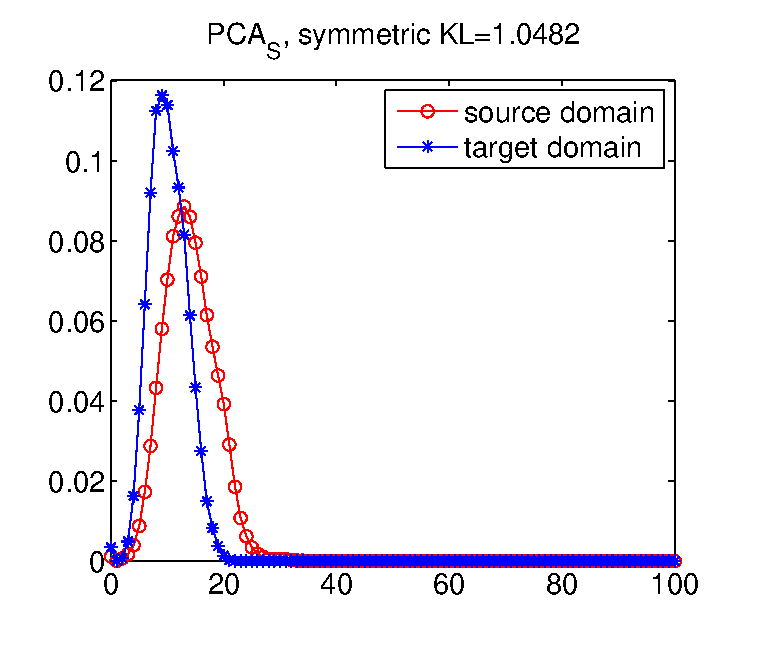
\includegraphics[width=0.45\columnwidth]{fig/fAWKLDistPCAs}
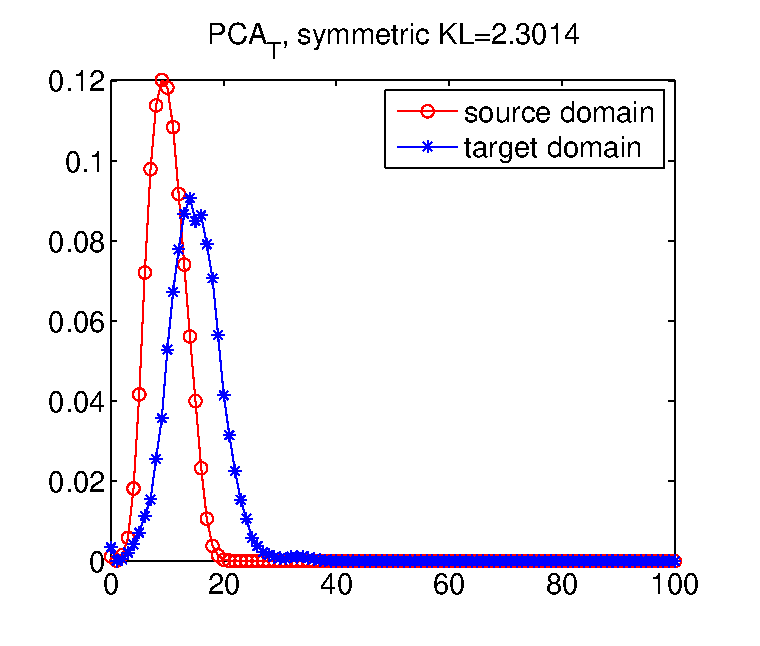
\includegraphics[width=0.45\columnwidth]{fig/fAWKLDistPCAt}\\
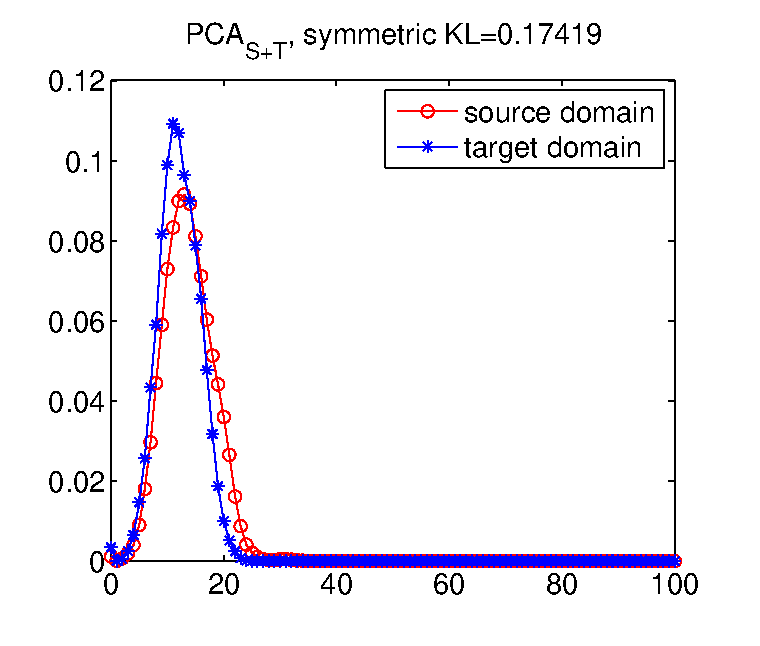
\includegraphics[width=0.45\columnwidth]{fig/fAWKLDistPCAst}
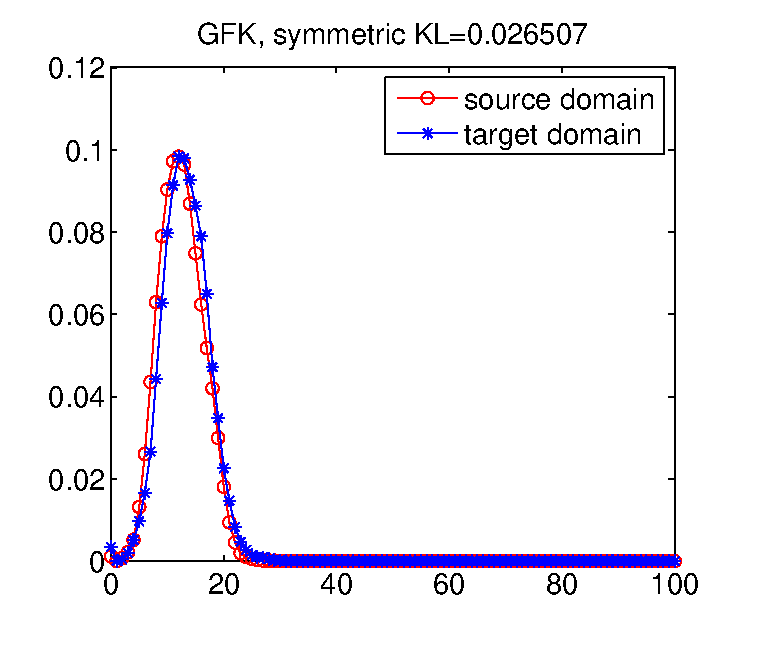
\includegraphics[width=0.45\columnwidth]{fig/fAWKLDistGFK}
\caption{Histograms of pairwise distances within each domain where the distances are calculated within four different subspaces. GFK induces  a subspace such that the difference between the source's histogram and the target's is the smallest.}
\label{fGFKKLDistance}
\end{figure}

\begin{table}
\centering
\caption{Symmetric KL divergences between the histograms of pairwise distances across two domains}
\label{tGFKKLDistance}
\begin{tabular}{|c|c|c|c|c|}\hline
Domain pairs & \PCAs & \PCAt & \PCAst & \GFK \\ \hline
\amazon - \caltech &  0.413 & 0.445 & 0.014 & 0.012 \\ \hline
\amazon - \dslr & 2.145 & 7.411 & 0.734 & 0.33 \\ \hline
\amazon - \webcam & 1.048 & 2.301 & 0.174 & 0.027 \\ \hline
\caltech - \dslr & 1.026 & 2.488 & 0.587 & 0.138 \\ \hline
\caltech - \webcam & 1.747 & 2.188 & 0.347 & 0.178 \\ \hline
\dslr - \webcam & 2.884 & 0.808 & 0.009 & 0.089 \\ \hline\hline
Average & 1.544 & 2.607 & 0.311 & \textbf{0.129} \\ \hline
\end{tabular}
\end{table}


Combining the results in Table~\ref{tDistPreserve} and~\ref{tGFKKLDistance}, we find that the GFK leads to a subspace that best satisfies the two desirable properties \emph{simultaneously}: minimal distortions to distances \textbf{and} matching how distances are distributed. This empirical evidence strongly supports the GFK as a method to extract domain-invariant features. This support is echoed by the superior performance of GFK in benchmark problems, reported in section~\ref{sExp}.
}



\subsubsection{GFK as a standalone approach to unsupervised domain adaptation}
We note that GFK entails domain-invariant features, since it ``averages out'' the domain idiosyncrasies by the intergation over the geodesic flow. As a result, we are able to directly use it to solve the unsupervised domain adaptation problem, in addition to employing it to build other algorithms (e.g., the landmark based method in the next section). Concretely, we  i) determine the optimal dimensionality of the subspaces either by the subspace disagreement measure~\cite{GongCVPR12Geodesic} or cross-validation; ii) compute the geodesic flow kernel $\mat{G}$ using the subspaces eq.~(\ref{eGFKDef}); iii) use the kernel to construct a classifier with  the labeled data, either using a kernelized classifier which requires only the inner products defined by the kernel matrix $\mat{G}$ or using the invariant features $\mat{L}\vct{x}$ in any other types of classifiers.% Experiments on visual object recognition (see section~\ref{eExp}) verify the effectiveness of GFK for solving unsupervised domain adaptation.% in the visual object recognition tasks. 
\newline \newline
{\bf Remark.} Gopalan \emph{et al.}'s work is the closest to our GFK approach in spirit \cite{gopalan2011domain}. They have also explored the idea of using geodesic flows to derive intermediate subspaces that interpolate between the source and target domains. A crucial difference from ours is that they sample a \emph{finite} number of subspaces and stack these subspaces into a very high-dimensional projection matrix. As such, the dimension of their features needs to be reduced. This extra step, unfortunately, might introduce modeling errors and practical challenges. For instance, it is not clear how to choose the subspace sampling rate or the right feature dimension after reduction. %and whether the dimension reduction method used there necessarily helps classification.

\eat{
In stark contrast, GFK is both conceptually and computationally simpler and eliminates the need to tune many hyper-parameters as by Gopalan \emph{et al.}'s approach. In particular, our kernel is in closed form, and computing it involves simple matrix algebra for example singular value decomposition. We have devised a fully automatic procedure, which is lacking in Gopalan \emph{et al.}'s work,  to choose the optimal dimensionality of the subspaces~\cite{GongCVPR12Geodesic}. {We also note that Zheng {\it et al.} proposed the same kernel, albeit independently and almost simultaneously~\cite{zheng2012grassmann}, though they did not offer an automatic procedure to determine the dimensions of the subspaces.}
}

% !TEX root = da.tex



\subsection{Landmarks for unsupervised domain adaptation}  \label{sLandmark}
One of the key challenges to unsupervised domain adaptation is that there is no labeled data in the target domain to train discriminative classifiers. We tackle this by the insight of landmarks --- some labeled instances in the source domain may be regarded as a subset drawn from the target. By automatically identifying those landmarks, we can thus approximate the discriminative loss of the target domain. 

As a motivating example for the landmarks, suppose the source domain contains furniture in a home environment  and the target domain consists of images of office-style furniture.  Conceivably, certain images from the source --- for instance those taken in home offices --- could also be regarded as samples from the target. Such images thus might have properties that are shared by both domains. These properties in turn can guide learning algorithms to search for invariant features or kernels.


%Our approach automatically identifies such images, which we call ``landmarks''.  We use them to bridge the source and target domains to generate multiple candidates of invariant feature spaces. Additionally, we exploit the {\em labels of the landmarks} to adapt the invariant features to be {\em discriminatively} optimal for the target domain, in contrast to GFK.  We also show that the landmark-based approach integrates well with GFK. In particular, our automatic landmark identification algorithm (section~\ref{sFindLandmark}) benefits significantly from using GFK as a similarity measure.

In the following, we give an overview of the landmark based approach, followed by details on how to identify landmarks. We then show how to exploit the landmarks for a series of GFKs and discriminative learning of kernels for the target domain.

\subsubsection{Overview of the landmark based approach to unsupervised adaptation}
As the first step, our landmark based approach plucks out and exploits the most desirable instances ---landmarks --- to facilitate adaptation. Identifying those instances requires comparing all possible subsets from the source domain to the target. We will show how this can be addressed with tractable optimization.

Leveraging the landmarks, we create a cohort of auxiliary tasks where landmarks explicitly bridge the source and target domains. Specifically, in those auxiliary tasks, the original target domain is augmented with landmarks, blurring the distinction across domains. Thus, those tasks are \emph{easier} to solve than the original domain adaptation problem. We show this is indeed true both theoretically and empirically. The auxiliary tasks offer multiple views of the original problem; they differ by how the landmarks are selected, which in turn are determined by the data pairwise similarities. In this work, we measure similarities at multiple scales (of distances). Thus, each task provides a different perspective to the adaptation problem, by being robust to idiosyncrasies in the domains at different granularities.


\begin{figure*}[t]
\centering
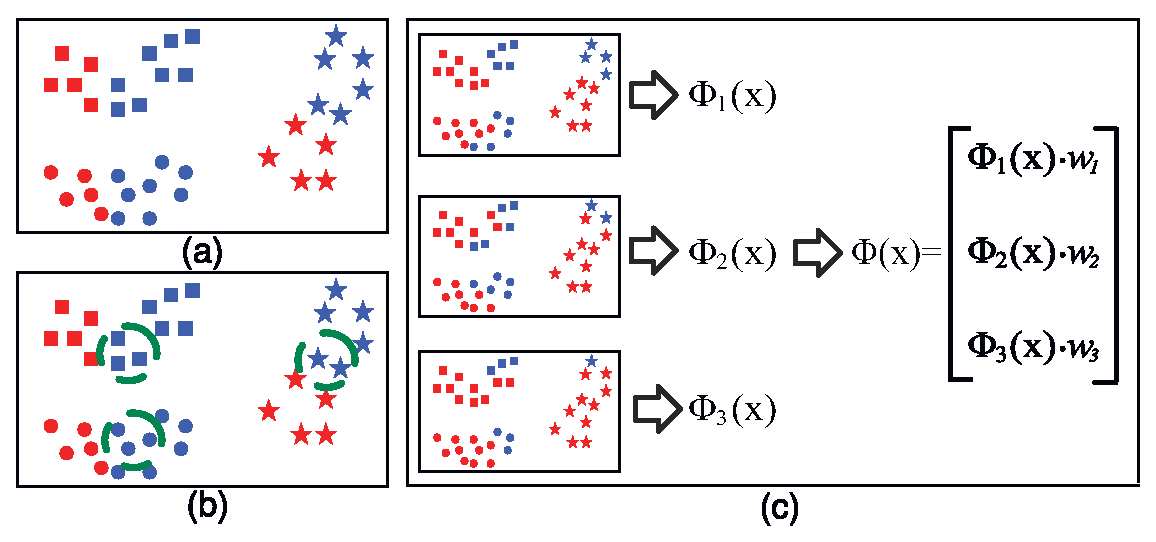
\includegraphics[width=0.8\columnwidth]{fig/fConcept1}
\caption{Main idea of our landmark based approach. (a) The original domain adaptation (DA) problem, where instances in red are from the target and in blue from the source. (b) \textbf{Landmarks}, shown inside the green circles, are data points from the source that can be regarded as samples from the target. (c) Multiple auxiliary tasks are created by augmenting the original target with landmarks, which switch their color (domain association) from blue to red. Each task gives rise to a new feature representation.  These representations are combined discriminatively to form domain-invariant features for the original DA problem. (best viewed in color)}
\label{fConcept}
\end{figure*}


The solutions of the auxiliary tasks give rise to multiple domain-invariant GFKs. We parameterize the invariant features for the original adaptation problem with those resultant kernels.  Intuitively, not all of the kernels are equally useful; to discern which are, we cast the corresponding  learning problem in terms of multiple kernel learning.  We learn the kernel discriminatively to  minimize classification errors on the landmark data instances, which serve as a proxy to discriminative loss on the target domain. Fig.~\ref{fConcept} schematically illustrates the overall approach.

%Despite such progress, existing approaches so far have only been limited to macroscopically examining the distribution similarity by tuning to statistical properties of the samples as a whole --- when comparing distributions, all the samples are used. This notion  is stringent, as it requires all discrepancies to  be accounted for and forces learning inefficiently (or even erroneously) from ``hard'' cases that might be just outliers to the target domains.

%In contrast, we will leverage the key insight that \textbf{\emph{not all instances are created equally in terms of adaptability}}. Thus, we will examine distribution similarity microscopically at the instance level;  In what follows,  we summarize the main idea behind our approach.  After describing it in detail in section~\ref{sApproach}, we contrast it to related work in section~\ref{sRelated}.


%We next describe our three-step landmark based approach. % below: i) identifying and selecting the landmark instances; ii) constructing multiple auxiliary tasks using the landmarks and inferring the corresponding domain-invariant feature spaces, one for each auxiliary task;   iii) discriminatively learning the final domain-invariant feature space that is optimized for the target domain.


\paragraph{\bf Step I: Discovering landmarks} \label{sFindLandmark}

Landmarks are data points from the source domain; however, given how they are distributed, they look like they could be samples from the target domain too (cf. Fig.~\ref{fConcept} for a schematic illustration, and Fig.~\ref{fLandmark} in section~\ref{sExp} for exemplar images identified as landmarks in vision datasets). The intuition behind our approach is to use these landmarks to bridge the source and the target domains.

\emph{How can we identify those landmarks?}  At first glance, it seems that we need to compare all possible subsets of training instances in the source domain to the target. We will show in the following this seemingly intractable problem can be relaxed and solved with tractable convex optimization.

Let $\src=\{(\vct{x}_{m},y_{m})\}_{m=1}^{\cst{M}}$ denote $\cst{M}$ data points and their labels from the source domain. Likewise, we use  $\tgt=\{\vct{x}_{n}\}_{n=1}^{\cst{N}}$ for the target domain.

{\bf Landmark selection.} To identify landmarks, we use  $\cst{M}$ indicator variables $\vct{\alpha}=\{\alpha_m \in \{0,1\}\}$, one for each data point in the source domain. If $\alpha_m = 1$, then $\vct{x}_m$ is regarded as a landmark. Our goal is to choose among all possible configurations of $\vct{\alpha}=\{\alpha_m\}$ such that the distribution of the \textbf{\emph{selected}} data instances is maximally similar to that of the target domain.

To determine whether the two distributions are similar, we use a non-parametric two-sample test called maximum mean discrepancy (MMD)~\cite{gretton2006kernel}. (Other approaches are also possible, including building density estimators when the dimensionality is not high.)  Specifically, we use a nonlinear feature mapping function $\phi(\cdot)$ to map $\vct{x}$ to a Reproducing Kernel Hilbert Space (RKHS) and compare the difference in sample means. {When the mapping function is a unit-ball in a universal RKHS, the difference can be conveniently calculated  in the following\footnote{The unit-ball condition allows the difference to be represented as a metric in the form of eq.~(\ref{eMMD}) and the universality ensures that the means are injective such that the difference in the means is zero if and only if the two distributions are the same. For more analysis, please refer to ~\cite{gretton2006kernel}.},
\begin{equation} \label{eMMD}
\mathsf{MMD}(\vct{\alpha}) = \left\| \frac{1}{\sum_m \alpha_m} \sum_m \alpha_m \phi (\vct{x}_m) - \frac{1}{\cst{N}} \sum_n \phi(\vct{x}_n)\right\|_{\mathcal{H}}^2,
\end{equation}
where $\sum \alpha_m$ is the number of selected landmarks, and the first term  inside the norm is the mean of the selected landmarks under the mapping.  

Our goal is to choose $\vct{\alpha}$ such that the difference is minimized. Furthermore, we impose the constraint that the labels are \emph{balanced} in the selected landmarks. Concretely, we arrive at the following optimization problem,
\begin{align} 
\min_{\vct{\alpha}}  \mathsf{MMD}(\vct{\alpha}) \qquad
\mathsf{s.t.} \quad \frac{1}{\sum_m \alpha_m} \sum_m \alpha_m y_{mc} = \frac{1}{{\cst{M}}}\sum_m y_{mc}, \label{eBalance}
\end{align}
where $y_{mc}$ is an indicator variable for $y_m = c$. The right-hand-side of the constraint is simply the prior probability of the class $c$, estimated from the source.}

We stress that the above criterion is defined on landmarks, which are a \emph{subset} of the source domain, as the sample mean is computed \emph{only} on the selected instances (cf. the denominator $\sum_m \alpha_m$ in eq.~(\ref{eBalance})).  This is very different from other approaches that have used similar non-parametric techniques for comparing distributions~\cite{tca,gretton09kmm}. There they  make stronger assumptions that all data points in the source domain need to be collectively distributed similarly to the target domain.  Furthermore, they do not impose the balance constraint of eq.~(\ref{eBalance}).  Our experimental results  show that these differences are crucial to the success of our approach.

Eq.~(\ref{eBalance}) is intractable due to the binary unknowns $\vct{\alpha}$. We relax and solve it efficiently by introducing new variables $\beta_m$ as $\alpha_m \left(\sum_m \alpha_m\right)^{-1}$.
We relax them to live on the simplex $\Delta=\{\vct{\beta}: \beta_m \ge 0, \sum_m \beta_m=1\}$. Substituting $\{\beta_m\}$ into eq.~(\ref{eBalance}) and its constraints, we arrive at the following {\em quadratic programming problem:}
\begin{equation}
\min_{\vct{\beta} \in \Delta}  \vct{\beta}\T \mat{A}\vct{\beta} - {2}/{\cst{N}}\, \vct{\beta}\T \mat{B} \vct{1} \qquad
\mathrm{ s.t.\ }   \sum_m \beta_m y_{mc} = {1}/{\cst{M}} \sum_m y_{mc},\ \ \ \forall\ c,
\label{eSelected}
\end{equation}
where $\mat{A} \in \R^{\cst{M}\times\cst{M}}$ denotes the positive semidefinite kernel matrix computed over the source domain, and $\mat{B} \in \R^{\cst{M}\times\cst{N}}$ denotes the kernel matrix computed between the source data points and target data points. We recover the binary solution for $\alpha_m$ by  finding the support of $\beta_m$, ie, $\alpha_m = \textsc{threshold}(\beta_m)$. In practice, we often obtain \emph{sparse} solutions, supporting our modeling intuition that only a subset of  instances in the source domain is needed to match the target domain.

{\bf Multiscale analysis.} The selection of landmarks depends on the kernel mapping $\phi(\vct{x})$ and its parameter(s). {To satisfy the requirement of being a unit-ball in a universal RKHS}, we use Gaussian RBF kernels, defined as follows:
\begin{equation} \label{eRBF}
K(\vct{x}_i, \vct{x}_j) = \exp\{  - (\vct{x}_i - \vct{x}_j)\T \mat{M} (\vct{x}_i - \vct{x}_j)/\sigma^2\},
\end{equation}
where the metric $\mat{M}$ is  positive semidefinite and we experiment with several choices.


The bandwidth $\sigma$ is a scaling factor for measuring distances and similarities between data points. Since we regard landmarks as likely samples from the target domain, the bandwidth $\sigma$ determines how much the source and the target are similar to each other at different granularities. A small $\sigma$ will attenuate distances rapidly and regard even close points as being dissimilar. As a result, the algorithm (eq.~(\ref{eBalance})) may select a \emph{large} number of points as landmarks in order to match the target distribution. A large $\sigma$ will have the opposite effect. Fig.~\ref{fLandmark}   illustrates the effect of $\sigma$.

Instead of choosing one scale $\sigma$ in the hope that it fits all, we devise a multiscale approach. We use a set $\{\sigma_q \in [\sigma_{min},\ \sigma_{max}]\}_{q=1}^{\cst{Q}}$. For each $\sigma_q$, we compute the kernel according to eq.~(\ref{eRBF}) and solve eq.~(\ref{eSelected}) to obtain the corresponding landmarks $\mathcal{L}^q = \{ (\vct{x}_m, y_m):  \alpha_m =1\}$.   Using multiple scales  adds the flexibility of modeling data where similarities cannot be measured in one homogeneous scale.  For example, the category of \textsc{grizzly bear} is conceivably much closer to \textsc{grey bear} than to \textsc{polar bear}, so to capture similarities among both the pairs as well as among all three, it is necessary to model them at two scales. Each set of landmarks (one set per scale) gives rise to a different perspective to the adaptation problem by suggesting which instances to explore to connect the source and the target. We achieve this connection by creating auxiliary tasks, as we describe next.

% in the next section, for each cohort of landmarks $\mathcal{L}^q$, we infer a new feature space $\mathcal{Z}^q$ that is domain-invariant if data is examined at the corresponding scale $\sigma^q$. These spaces will be combined nonlinearly and discriminatively to yield a final feature space for domain adaptation (cf. section~\ref{sMKL}).

%We denote all the landmarks collectively  by $\{\landmark\}_{q=1}^\cst{Q}$.  %Intuitively, each $\landmark$ includes the data points from the source which looks like from the target domain, at that scaling.


%In this paper, we focus on using Gaussian RBF style kernels to select landmarks.  Measuring the distance  between $\vct{x}_i$ and $\vct{x}_j$ with respect to a metric $\mat{M}$ as
%\begin{equation}
%d_{\mat{M}}^2 (\vct{x}_i, \vct{x}_j) = (\vct{x}_i - \vct{x}_j)\T \mat{M} (\vct{x}_i - \vct{x}_j),
%\label{eDist}
%\end{equation}
%the corresponding Gaussian kernel uses the bandwidth as a scaling parameter to transferorm distances between data points  into similarity measure

%A large bandwidth $\sigma^2$ will attenuate distances slower and treat distant points being similar. A small bandwidth attenuates distances rapidly and will only treat points in close neighborhood as being similar. In other words, the bandwidth



\paragraph{\bf Step II: Constructing auxiliary tasks} \label{sAuxiliary}
Imagine we create a new source domain $\src^q = \src \setminus \landmark$ and a new target domain $\tgt^q = \tgt\bigcup \landmark$, where the landmarks $\landmark$ are removed from and added to the source and target domains, respectively. The landmarks' labels are not used yet at this stage.

Our auxiliary tasks are defined as $\cst{Q}$  domain adaptation problems, $\src^q \rightarrow \tgt^q$. The auxiliary tasks differ from the original problem $\src \rightarrow \tgt$ in an important aspect:
the new tasks should be ``easier'', as the existence of landmark points ought to aid the adaptation. This is illustrated by the following theorem, stating that the discrepancy between the new domains is smaller than the original.

Let $P_S(X)$ and $P_T(X)$ denote the distributions of the original source and target domains, respectively. Suppose $P_S(X)= \alpha P_N(X) + (1-\alpha)P_L(X)$ with $\alpha \in [0, 1)$ is a mixture model where $P_L(X)$ is the component corresponding to the landmark data points and $P_N(X)$ corresponds to the distribution of the non-landmark instances.  For the auxiliary task, assume the new target distribution is modeled as a mixture distribution $Q_T(X) =  \beta P_T(X) + (1-\beta) P_L(X)$ where $\beta \in [0,\ 1)$. Furthermore, assume the source distribution remains essentially unchanged, which is easily satisfied as long as the number of instances in the source domain is significantly greater than the number of landmark instances and the landmarks are selected \emph{i.i.d.} from $P_L(X)$\footnote{Note that we do not require the landmarks to be \emph{i.i.d} samples from $P_S(X)$ --- they only need to be representative samples of $P_L(X)$.}. In what follows, we omit the arguments $(X)$ to simplify the notation.

\begin{thm}
\label{thAux}
The following inequality holds,
\begin{equation}
 KL( P_S  \|  Q_T ) \le  KL( P_S \|  P_T)  \notag
\end{equation}
where $KL(\cdot\|\cdot)$ stands for the Kullback-Leibler divergence, if %the following condition is satisfied
\begin{align} \label{eAssumption}
\alpha KL(P_N\|P_{T})+(1-\alpha)KL(P_L\|P_{T}) 
    \geq {9}/{8}\max \left\{ KL(P_L\|P_N),\, KL(P_N\|P_L) \right\}.
\end{align}In words, the new target distribution is closer to the source distribution, on the condition that the inter-domain difference (i.e. the left-hand-side) is greater than the intra-domain discrepancy or inhomogeneity (i.e., the right-hand-side).
\end{thm}
The proof is in the Appendix of~\cite{GongIJCV14Learning}. Note that the condition in eq.~(\ref{eAssumption}) is mild:  we expect the source domain is relatively homogeneous and is distinct from the target. With the reduced discrepancy between $P_S(X)$ and $Q_T(X)$, we can apply the analysis in~\cite[Lemma~1]{mansour09multiple} to show that classifiers applied to $Q_T(X)$ attain a smaller generalization error bound than those applied to $P_T(X)$.

These insights motivate our design of auxiliary tasks: they conceivably have low accuracy for binary classification as the landmarks blend the two domains, discouraging the use of domain-specific features.  We describe next how to extract domain-invariant kernels/features using the solutions of those easy problems as a \emph{basis}.

{\bf Learning basis from auxiliary tasks.} {Having shown that the auxiliary tasks represent easier domain adaptation problems, we now use them for adaptation.  Specifically,} for every pair of auxiliary domains, we use the geodesic flow kernel to compute domain-invariant features. The GFK is particularly adept at measuring domain-invariant distances among data points, as exemplified by its superior performance in nearest-neighbor classifiers (cf. section~\ref{sGFKResults}). Thus, it is especially suitable for the final stage of our approach when we compose complex domain-invariant features (cf. section~\ref{sMKL}). The domain-invariant feature space is extracted as the mapping $\Phi_q(\vct{x}) = \mat{L}_q\vct{x}$, where $\mat{G}_q=\mat{L}_q\T\mat{L}_q$ is the GFK for the $q$-th auxiliary task (cf. eq.~(\ref{eGFKInvariant})).  In the following, we describe how to integrate the spaces --- one for each auxiliary task --- \emph{discriminatively} so that the final feature space is optimal for the target.

\paragraph{\bf Step III: Discriminative learning of kernels and classifiers} \label{sMKL}

In this final step, we reveal the second use of landmarks beyond constructing auxiliary tasks. We will use their labels to learn  \emph{discriminative} domain-invariant features for the target domain. Concretely, we compose the features for the original adaptation problem with the auxiliary tasks' features as a basis.

We scale and concatenate those features $\{\sqrt{w_q}\Phi_q(\vct{x})\}_{q=1}^{\cst{Q}}$  into a ``super'' vector $\vct{f}$. Learning $\{w_q\}$ is cast as learning a convex combination of all kernels $\mat{G}_q$ \cite{lanckriet04kernel},
\begin{equation}
\mat{F} = \sum_q w_q \mat{G}_q,\qquad \  \mathrm{s.t.}\ \ \ w_q \ge 0\ \mbox{and}\ \sum_q w_q = 1.
\label{eMKL}
\end{equation}
We use the kernel $\mat{F}$ in training a SVM classifier and the labels of the landmarks $\{\landmark\}$, i.e., $\mkltrain = \sum_q \landmark$ to optimize $\{w_q\}$ discriminatively.  We use $\mkltest = \src \setminus \mkltrain$ as the validation dataset for model selection.  Since $\mkltrain$ consists of landmarks that are distributed similarly to the target, we expect the classification error on $\mkltrain$ to be a good proxy to that of the target.

%Multiple kernel learning formulations such as eq.~(\ref{eMKL}) often yield sparse solutions where some optimal coefficients $w_q$ are zeroes. Thus, the discriminative learning prunes away scales that are not informative. Our experimental results verify that (cf. the Supplementary Material).


\eat{
\subsection{Summary}

To recap our landmark-based approach: i) at each scale $\sigma_q$ and with the aid of GFK, we automatically select \emph{landmark} instances that are distributed similarly to the target; ii) we then construct \emph{auxiliary} tasks and use their solutions as a basis to compose domain-invariant features; iii)  we learn features \emph{discriminatively}, using classification loss on the landmarks as a proxy to the discriminative loss on the target.  %by augmenting the target domain with those landmarks, which aid adaptation. Morever, the solutions to the auxiliary tasks are domain-invariant features that are informative for the original task. iii) those features are discriminatively combined

 in the following: i) for each scale $\sigma_q$,  identify  the set of landmark points $\landmark$ by solving the convex optimization problem eq.~(\ref{eSelected});
ii) for each $\landmark$, construct the corresponding auxiliary task and derive a kernel $\mat{G}_q$ using the method described in section~\ref{sAuxiliary};
iii) formulate the multiple kernel learning problem, and compute the optimal combination coefficients as in eq.~(\ref{eMKL}) to combine the kernels $\mat{G}_q$. The resulting kernel $\mat{F}$ encodes the final domain-invariant feature space.

We emphasize that our approach differs from conventional approaches for learning domain-invariant features \cite{xxx}. In those approaches, invariant features are first learned without using labels and then a classifier is learned with labeled data. One disadvantage of that two-stage paradigm is that the invariant features are \emph{not} optimized to be discriminative. In contrast,
our approach is one-stage:  the combined kernel $\mat{F}$ encodes the invariant features and are trained \emph{discriminatively} with labeled data. Thus, after learning, the domain-invariant features are likely to perform well.
}



%%%%%%%%%%%%%%% OLD TEXT



% !TEX root = da.tex
\section{Experiments} \label{sExp}

\begin{figure*}[t]
  \centering
      \includegraphics[width=0.9\columnwidth]{fig/fMonitor.eps} \\
    \caption{Example images from Caltech-256, Amazon, DSLR, and Webcam. Caltech and Amazon images are mostly from online merchants, while DSLR and Webcam images are  from offices. }\label{fMonitor}
\end{figure*}

We evaluate our methods in the context of visual object recognition; more results for other tasks (e.g., text analyses) are shown in a prior conference paper~\cite{gong13landmark}. We describe the general experimental setup first, and then report the results of our GFK and landmark based approaches to domain adaptation.
%After describing the general experimental setup in section~\ref{sSetup}, we report first the recognition results of applying our geodesic flow kernel (GFK) approach (section~\ref{sGFKResults}), followed by the results from our landmark-based approach (section~\ref{sLandmarkResults}). While the landmark-based approach in general outperforms GFK on the benchmark datasets we have tested, we believe that the method of GFK can stand alone separate from the landmarks idea, making its results interesting and valuable in their own right. In particular, the kernel function can be used as a building block for other methods, as exemplified by our success with the landmark approach.
\eat{
We also investigate other practical issues in applying domain adaptation techniques to real-world problems. In addition to improving visual object recognition for a pair of \emph{given} source and target domains, we also study how we can select which source domain to pair with the target domain, given multiple source domains and a target domain. To this end, we  introduce a metric called Rank of Domain (ROD) that can be used to rank a list of source domains based on how suitable they are to domain adaptation. We describe the metric and its application in section~\ref{sROD}.

Finally, as a novel application of domain adaptation techniques, we investigate the
\emph{dataset bias} problem, recently studied in \cite{TorralbaCVPR11Unbiased}. Through their analysis, the authors identified a few datasets of high ``market value'', suggesting that they are  less biased, and more representative of real-world objects. We re-examine these datasets with a new perspective: \emph{are such high-valued datasets indeed useful in improving a target domain's performance?} Our analysis suggests it would be beneficial to also consider ``ease of adaptability'' in assessing the value of datasets. We describe our findings in section~\ref{sAdaptability}.
}

{\bf Datasets.} We use the three datasets studied in~\cite{saenko2010adapting} in our experiments: Amazon (images downloaded from online merchants), Webcam (low-resolution images by a web camera), and DSLR (high-resolution images by a digital SLR camera).  Additionally, to validate the proposed methods on a wide range of datasets, we added Caltech-256~\cite{Caltech256} as the fourth dataset. We regard each dataset as a domain, and extract 10 classes common to all datasets: \textsc{backpack, touring-bike, calculator, head-phones, computer-keyboard, laptop-101, computer-monitor, computer-mouse, coffee-mug,} and \textsc{video-projector}.  There are 8 to 151 samples per category per domain, and 2533 images in total. Fig.~\ref{fMonitor} highlights the differences among these domains  with example images from the \textsc{monitor} class. We report our results on adapting 10-way classification between the four domains\footnote{In the supplementary material of our previously published work~\cite{gong12gfk}, we report the results on  all the 31 categories common to Amazon, Webcam and DSLR. There demonstrates the same trend, that our proposed methods significantly outperform competing approaches.}. We obtain the results of the competing methods by rerunning publicly available code or our implementation if the code is unavailable.

{\bf Features.} We follow similar feature extraction and experiment protocols used in previous work. Briefly, we use SURF features \cite{bay2006surf} and encode the images with 800-bin histograms with the codebook trained from a subset of Amazon images. The histograms are normalized first and then z-scored to  have zero mean and unit standard deviation in each dimension. We share our features (and code) publicly to promote direct reproducibility of our results\footnote{Features and code of our methods: \url{http://www-scf.usc.edu/~boqinggo/da.html}.}.

{\bf Training settings.} For experiments using GFK for adaptation, we conduct experiments in 20 random trials for each pair of source and target domains.  In each trial, we randomly sample labeled data in the source domain as training examples, and unlabeled data in the target domain as testing examples. This setting is in accordance with prior work~\cite{saenko2010adapting,kulisyou,gopalan2011domain} and provides the maximal comparability to those methods. More details on how data are split are provided in the next section. We report averaged accuracies on target domains as well as standard errors.  For GFK results, 1-nearest neighbor is used as our classifier as it does not require cross-validating parameters.  For our algorithms,  the dimensionalities of subspaces are selected according to the subspace disagreement measure in~\cite{GongCVPR12Geodesic}.  For the hyper-parameters of the methods we compare to, we use what are recommended in the published work.

For experiments using our landmark-based approach for adaptation, we use all training instances from the source domains. Except this difference, other training setups are the same as for the experiments using GFK.




\begin{table}[t]
\centering 
\caption{Recognition accuracies on target
domains with \emph{unsupervised} adaptation  via GFK. (C: Caltech, A: Amazon, W: Webcam, and D: DSLR)}  \label{tUnsuper-Caltech2}
\begin{tabular}{lcccccccccccc} \toprule
 Method  & C$\rightarrow$A & C$\rightarrow$W & C$\rightarrow$D
& A$\rightarrow$C & A$\rightarrow$W & A$\rightarrow$D &
W$\rightarrow$C & W$\rightarrow$A & W$\rightarrow$D &
D$\rightarrow$C & D$\rightarrow$A & D$\rightarrow$W\\ \midrule
\OrigFeat & 20.8 & 19.4 & 22.0 &
22.6 & 23.5 & 22.2 & 16.1 &
20.7 & 37.3 & 24.8 & 27.7 &
53.1\\ 
\midrule
\PCAs & 34.7 &
{\color{blue}{\underline{\emph{31.3}}}} & 33.6 &
34.0 & 31.3 & 29.4 & 23.4 &
28.0 & 68.2 & 26.8 & 28.1 &
61.7\\ 
\PCAt   &
{\color{blue}{\underline{\emph{37.5}}}} &
{\color{red}\textbf{33.9}}&
{\color{blue}{\underline{\emph{37.8}}}} &
{\color{blue}{\underline{\emph{35.4}}}} &
{\color{red}\textbf{34.9}} &
{\color{blue}{\underline{\emph{33.3}}}} &
{\color{red}\textbf{29.6}} &
{\color{blue}{\underline{\emph{32.5}}}} & 67.4 &
{\color{blue}{\underline{\emph{31.2}}}} & {\color{blue}{\underline{\emph{34.4}}}} & {\color{red}\textbf{79.4}}\\
\PCAst  & {\color{blue}{\underline{\emph{36.6}}}} &
{\color{blue}{\underline{\emph{32.1}}}} & 34.9 &
{\color{blue}{\underline{\emph{35.8}}}} &
{\color{blue}{\underline{\emph{32.8}}}} & 31.5 &
{\color{blue}{\underline{\emph{28.1}}}} &
{\color{blue}{\underline{\emph{31.6}}}} &
{\color{red}\textbf{74.1}} &
{\color{blue}{\underline{\emph{30.8}}}} & 33.3 & {\color{red}\textbf{79.7}}\\
\PLSs & 26.7 & 26.0 & 28.2 &
31.1 & 29.3 & 28.0 & 18.3&
21.1 & 42.8 & 21.4 & 26.5 &
41.9\\ 
\midrule
\ICCV~(impl.)  &
{\color{blue}{\underline{\emph{36.8}}}} &
{\color{blue}{\underline{\emph{30.6}}}} & 32.6 &
{\color{blue}{\underline{\emph{35.3}}}} & 31.0 &
30.7 & 21.7 & 27.5 & 54.3 &
29.4 & 32.0 & 66.0\\
 \ICCV~(opti.) &
{\color{blue}{\underline{\emph{36.9}}}} &
{\color{red}\textbf{33.9}} & 35.2 &
{\color{blue}{\underline{\emph{35.6}}}} &
{\color{red}\textbf{34.4}} &
{\color{red}\textbf{34.9}} &
{\color{blue}{\underline{\emph{27.3}}}} &
{\color{blue}{\underline{\emph{31.3}}}} &
{\color{blue}{\underline{\emph{70.7}}}} & 30.0 &
32.6 & {\color{blue}{\underline{\emph{74.9}}}}\\
\midrule
{\GFK}~(A,A) & {\color{blue}{\underline{\emph{36.9}}}}
& {\color{red}\textbf{33.7}} & 35.2 &
{\color{blue}{\underline{\emph{35.6}}}} &
{\color{red}\textbf{34.4}} &
{\color{red}\textbf{35.2}} &
{\color{blue}{\underline{\emph{27.2}}}} &
{\color{blue}{\underline{\emph{31.1}}}} &
{\color{blue}{\underline{\emph{70.6}}}} & 29.8 &
32.5 & {\color{blue}{\underline{\emph{74.9}}}}\\
{\GFK}~(S,A) & {\color{red}\textbf{40.4}} &
{\color{red}\textbf{35.8}} &
{\color{red}\textbf{41.1}} &
{\color{red}\textbf{37.9}} & {\color{red}\textbf{35.7}} &
{\color{red}\textbf{35.1}} &
{\color{red}\textbf{29.3}} &
{\color{red}\textbf{35.5}} &
{\color{blue}{\underline{\emph{71.2}}}} &
{\color{red}\textbf{32.7}} & {\color{red}\textbf{36.2}} & {\color{red}\textbf{79.1}}\\ 
\bottomrule
\end{tabular}

\vspace{10pt}

\caption{Recognition accuracies on target
domains with \emph{supervised} adaptation via GFK and ``deep'' \textsc{DeCAF} features~\cite{DonahueX13Decaf}. (C: Caltech, A:
Amazon, W: Webcam, and D: DSLR)} \label{tDeepGFK}
\begin{tabular}{lcccccccccccc} 
\toprule
Method &  C$\rightarrow$D & C$\rightarrow$W & C$\rightarrow$A &
A$\rightarrow$C & A$\rightarrow$W & A$\rightarrow$D &
W$\rightarrow$C & W$\rightarrow$A & W$\rightarrow$D &
D$\rightarrow$C & D$\rightarrow$A & D$\rightarrow$W\\
\midrule
{\GFK}~(S,A) & && && &&&&& &  & \\
\textsc{w/ DeCAF} & 89.5 &
 79.5 &
85.3 &
81.4 &
77.3 &
84.5 &
74.7 &
84.2 &
99.5 &
76.6 &
76.9 &
97.3\\
\bottomrule
\end{tabular}

\end{table}


\subsection{Adaptation via GFK} \label{sGFKResults}

We compare our methods with various baseline and competing approaches: (1)\, \OrigFeat\ where we use the original features, i.e.,  without learning any new representations for domain adaptation; (2)
\PCAs\ where we project the original features into the PCA subspace learned from the \emph{source} domain; (3) \PCAt\ where  we project the original features into the PCA subspace learned from the \emph{target} domain; (4)
\PCAst\ where the PCA subspace is learned from  the \emph{combined} data of both the source and target domains; (5) \PLSs\ where  we project the original features into the Partial Least Squares (PLS)~\cite{PLS} subspace computed using the source domain's labels. %PLS is similar to PCA except it takes label information into consideration, and thus can be seen as a form of supervised dimensionality reduction \cite{PLS}.

We also implement the method in \cite{gopalan2011domain}. We refer to it as the geodesic flow sampling approach ({\ICCV}). While it also uses geodesic flows to model domain mismatch, the approach \emph{samples} a finite number of subspaces and uses them to construct high-dimensional features, followed by dimensionality reduction and classification. As the authors of this method suggest, we use PCA subspaces for both domains. We report results on two variants: i)  our implementation using the recommended parameters reported in \cite{gopalan2011domain}, such as the number of sampled subspaces and the reduced dimensionality (denoted {\ICCV}~(impl.)), and ii) our implementation using the optimal dimensionality automatically selected by our algorithm ({\ICCV}~(opti.)).

For our approach, we use two types of subspaces for the source data: {\PCAs} and {\PLSs}.  For the target domains, we use only {\PCAt}  as there are no labels. Thus, there are two variants of our  method: {\GEO} and {\plsGEO}.


Table \ref{tUnsuper-Caltech2} summarizes the classification accuracies as well as standard errors of all the above methods for different pairings of the source and target domains. Note that, to fit the table within the width of the page, we have shortened {\GEO} to {\GFK(A,A)}, and {\plsGEO} to {\GFK(S,A)}. The best group  (differences up to one standard error) in each column is in bold font and the second best group (differences up to one standard error)  is in italics and underlined.

All domain adaptation methods improve the accuracies over the baseline \OrigFeat. Further, our {\GFK} based methods in general outperform\ \ICCV.  Moreover, {\plsGEO} performs the best. Two key factors may contribute to the superiority of our method: i) the kernel integrates all the subspaces along the flow, and is hence able to model better the domain shift between the source and the target; ii) this method uses a discriminative subspace (by PLS) in the source domain to incorporate the label information. This has the benefit of avoiding projection directions that contain noise and very little useful discriminative information. PCA,  on the other hand, does not always yield subspaces that contain discriminative information. %Consequently all the improvements by our {\plsGEO} over {\ICCV}  are statistically significant, with margins more than one standard error.


It is also interesting to note that the PCA-based baselines, especially {\PCAst} and {\PCAt}, perform quite well. They are often in the second-best performing group, and are even better than the {\ICCV} methods on DLSR $\rightarrow$ Webcam and Webcam $\rightarrow$ DSLR.  We suspect that because the domain difference between DSLR and Webcam is small, either {\PCAt} or {\PCAst} is already able to capture the commonness of the two domains well. For instance, both DSLR and Webcam contain similar office images though with different resolutions  (see Fig.~\ref{fMonitor} for an example). %The similarity between Webcam and DSLR is also confirmed by our ROD metric, which we will describe in section~\ref{sROD}.
\newline \newline \noindent 
{\bf GFK with ``deep'' features.} Deep learning has been shown very effective for a variety of computer vision tasks. Table~\ref{tDeepGFK} are the results of GFK with the deep \textsc{DeCAF} features~\cite{DonahueX13Decaf}. The experiment setup remains the same as before except that, in each of the 20 random rounds, we use the remaining source data as the validation set to choose the subspace dimension --- since the \textsc{DeCAF} features are very high dimensional, the subspace disagreement measure~\cite{GongCVPR12Geodesic} is always below the threshold 1. The selected subspace dimensions are between 10 and 40. Comparing Tables~\ref{tUnsuper-Caltech2} and \ref{tDeepGFK}, we can see that the deep features significantly outperform the handcrafted SURF features for the unsupervised domain adaptation.


\eat{
In the last row of 
In semi-supervised adaptation, we have a small labeled set of target data for training classifiers. Additionally, it is straightforward to take advantage of the labeled target data to extend GFK by constructing the Partial Least Square subspace estimated on the target domain, i.e., \plsGEOpls.  Table \ref{tSemi-Caltech} shows the results of all methods, including an extra competing metric learning method {\ECCV} \cite{saenko2010adapting}, which uses the correspondence between source and target labeled data to learn a Mahalanobis metric. Our {\plsGEO} is still the best, followed by {\GEO}. Note that though  {\plsGEOpls} incorporates  discriminative information from both domains, it does not perform as well as {\plsGEO}. This is probably  due to the lack of enough labeled data in the target domains to give a reliable estimate of the PLS subspaces. %The  {\ECCV} method does not perform well either, probably due to the same reason.
}

\eat{
For a given target domain, there is a preferred source domain which leads to the best performance, either using {\OrigFeat} or  any of the domain adaptation methods. For example, for the domain Webcam, the source domain DSLR is better than the domain Amazon. This might be attributed to the similarity in DSLR and Webcam, illustrated in Fig.~\ref{fMonitor}. We analyze this in detail in section~\ref{sROD}.
}


 

\eat{
\begin{sidewaystable}
\centering
\caption{Recognition accuracies on target
domains with \emph{semi-supervised} adaptation via GFK (C: Caltech, A:
Amazon, W: Webcam, and D: DSLR).} \label{tSemi-Caltech}
\begin{tabular}{|c|c|c|c|c|c|c|c|c|c|c|c|c|}\hline
Method &  C$\rightarrow$D & C$\rightarrow$W & C$\rightarrow$A &
A$\rightarrow$C & A$\rightarrow$W & A$\rightarrow$D &
W$\rightarrow$C & W$\rightarrow$A & W$\rightarrow$D &
D$\rightarrow$C & D$\rightarrow$A & D$\rightarrow$W\\
\hline \hline
\OrigFeat & 26.5$\pm$0.7 & 25.2$\pm$0.8 & 23.1$\pm$0.4 &
24.0$\pm$0.3 & 31.6$\pm$0.6 & 28.1$\pm$0.6 & 20.8$\pm$0.5 &
30.8$\pm$0.6 & 44.3$\pm$1.0 & 22.4$\pm$0.5 & 31.3$\pm$0.7 &
55.5$\pm$0.7\\
\hline \hline
\PCAs &
{\color{blue}{\underline{\emph{48.9}}}}$\pm$1.0 &
{\color{blue}{\underline{\emph{54.2}}}}$\pm$0.9 & 40.3$\pm$0.4 &
35.5$\pm$0.5 & 47.3$\pm$0.7 &
{\color{blue}{\underline{\emph{47.8}}}}$\pm$1.0 & 28.1$\pm$0.8 &
38.2$\pm$0.6 & 72.1$\pm$0.8 & 27.0$\pm$0.5 & 36.8$\pm$0.5 &
64.4$\pm$0.7\\
\hline
\PCAt   & {\color{blue}{\underline{\emph{49.9}}}}$\pm$0.8 & 52.1$\pm$0.8 &
{\color{blue}{\underline{\emph{41.7}}}}$\pm$0.4 & {\color{blue}{\underline{\emph{37.6}}}}$\pm$0.4 &
51.8$\pm$0.8 & 44.1$\pm$1.0 & {\color{red}\textbf{33.9}}$\pm$0.6 &
41.5$\pm$0.5 & 70.0$\pm$0.7 &
{\color{red}\textbf{34.1}}$\pm$0.4 & {\color{blue}{\underline{\emph{42.1}}}}$\pm$0.4 & {\color{blue}{\underline{\emph{81.3}}}}$\pm$0.4\\
\hline
\PCAst  & {\color{blue}{\underline{\emph{48.7}}}}$\pm$1.2 &
{\color{blue}{\underline{\emph{55.8}}}}$\pm$0.9 & {\color{blue}{\underline{\emph{42.0}}}}$\pm$0.6 &
{\color{blue}{\underline{\emph{37.7}}}}$\pm$0.4 & 49.8$\pm$1.0 &
{\color{blue}{\underline{\emph{47.5}}}}$\pm$1.2 &
{\color{red}\textbf{33.6}}$\pm$0.7 &
{\color{blue}{\underline{\emph{42.9}}}}$\pm$0.6 &
{\color{red}\textbf{77.1}}$\pm$0.6 &
{\color{red}\textbf{34.0}}$\pm$0.4 & {\color{blue}{\underline{\emph{42.9}}}}$\pm$0.5 & {\color{red}\textbf{83.0}}$\pm$0.4\\
\hline \hline
\PLSs &
43.1$\pm$1.0 & 45.9$\pm$1.0 &
36.8$\pm$0.5 & 31.4$\pm$0.6 & 41.4$\pm$0.9 & 45.5$\pm$1.1 &
24.7$\pm$0.7 & 32.2$\pm$0.9 & 49.1$\pm$0.9 & 26.0$\pm$0.8 &
34.5$\pm$0.4 & 49.4$\pm$1.2\\
\hline
\PLSt   & 27.3$\pm$1.1 &
25.3$\pm$0.4 & 28.9$\pm$0.6 & 26.3$\pm$0.3 & 23.6$\pm$0.9 &
28.0$\pm$1.0 & 22.2$\pm$0.4 & 25.2$\pm$0.9 & 47.0$\pm$1.2 &
25.8$\pm$0.4 & 27.9$\pm$0.4 & 47.1$\pm$0.9\\
\hline \PLSst & 36.9$\pm$0.9 & 37.0$\pm$0.9 & 33.5$\pm$0.5 &
32.4$\pm$0.4 & 35.6$\pm$1.1 & 36.9$\pm$1.2 & 25.4$\pm$0.8 &
31.6$\pm$0.6 & 52.1$\pm$1.2 & 27.5$\pm$0.7 & 32.9$\pm$0.6 &
53.1$\pm$1.2\\ \hline \hline {\ECCV} (impl.) & 35.0$\pm$1.1 & 34.7$\pm$1.0
& 33.7$\pm$0.8 & 27.3$\pm$0.7 & 36.0$\pm$1.0 & 33.7$\pm$0.9 & 21.7$\pm$0.5
& 32.3$\pm$0.8 & 51.3$\pm$0.9 & 22.5$\pm$0.6 & 30.3$\pm$0.8 & 55.6$\pm$0.7\\
 \hline \ICCV (impl.)& 36.6$\pm$0.8 &
37.2$\pm$0.9 & 40.2$\pm$0.7 &
{\color{blue}{\underline{\emph{37.7}}}}$\pm$0.5 & 37.9$\pm$0.7 &
34.5$\pm$1.1 & 29.2$\pm$0.7 & 38.2$\pm$06 & 60.6$\pm$1.0 &
30.2$\pm$0.7 & 39.2$\pm$0.7 & 69.5$\pm$0.9 \\ \hline {\ICCV
(opti.)}& {\color{blue}{\underline{\emph{50.2}}}}$\pm$0.8 &
{\color{blue}{\underline{\emph{54.2}}}}$\pm$0.9 &
{\color{blue}{\underline{\emph{42.0}}}}$\pm$0.5 &
{\color{blue}{\underline{\emph{37.5}}}}$\pm$0.4 &
{\color{blue}{\underline{\emph{54.2}}}}$\pm$0.8 &
{\color{blue}{\underline{\emph{46.9}}}}$\pm$1.1 &
{\color{red}\textbf{32.9}}$\pm$0.7 &
{\color{blue}{\underline{\emph{43.0}}}}$\pm$0.7 &
{\color{blue}{\underline{\emph{75.2}}}}$\pm$0.7 &
{\color{blue}{\underline{\emph{32.9}}}}$\pm$0.4 & {\color{red}\textbf{44.9}}$\pm$0.7 & 78.6$\pm$0.4\\
\hline
{\GFK}(A,A) & {\color{blue}{\underline{\emph{49.5}}}}$\pm$0.9
& {\color{blue}{\underline{\emph{54.2}}}}$\pm$0.9 &
{\color{blue}{\underline{\emph{42.0}}}}$\pm$0.5 &
{\color{blue}{\underline{\emph{37.8}}}}$\pm$0.4 &
{\color{blue}{\underline{\emph{53.7}}}}$\pm$0.8 &
{\color{blue}{\underline{\emph{47.0}}}}$\pm$1.2 &
{\color{red}\textbf{32.8}}$\pm$0.7 &
{\color{blue}{\underline{\emph{42.8}}}}$\pm$0.7 &
{\color{blue}{\underline{\emph{75.0}}}}$\pm$0.7 &
{\color{blue}{\underline{\emph{32.7}}}}$\pm$0.4 & {\color{red}\textbf{45.0}}$\pm$0.7 & 78.7$\pm$0.5\\
\hline
{\GFK}(S,A) &{\color{red}\textbf{55.0}}$\pm$0.9 &
{\color{red}\textbf{57.0}}$\pm$0.9 &
{\color{red}\textbf{46.1}}$\pm$0.6 &
{\color{red}\textbf{39.6}}$\pm$0.4 &
{\color{red}\textbf{56.9}}$\pm$1.0 &
{\color{red}\textbf{50.9}}$\pm$0.9 &
{\color{blue}{\underline{\emph{32.3}}}}$\pm$0.6 &
{\color{red}\textbf{46.2}}$\pm$0.7 &
{\color{blue}{\underline{\emph{74.1}}}}$\pm$0.9 &
{\color{red}\textbf{33.9}}$\pm$0.6 & {\color{red}\textbf{46.2}}$\pm$0.6 & 80.2$\pm$0.4\\
\hline
{\GFK}(S,S) &38.6$\pm$1.4 & 34.0$\pm$0.9 & 38.7$\pm$0.6
& 36.6$\pm$0.4 & 36.3$\pm$0.9 & 34.1$\pm$1.0 & 28.6$\pm$0.6 &
36.3$\pm$0.5 & 68.6$\pm$1.0 &
{\color{blue}{\underline{\emph{32.6}}}}$\pm$0.4 & 35.0$\pm$0.4 &
74.6$\pm$0.5\\ \hline
\end{tabular}
\end{sidewaystable}
}




\eat{
\paragraph{Automatic inferring the dimensionality of subspaces}

\begin{figure*}
\centering
    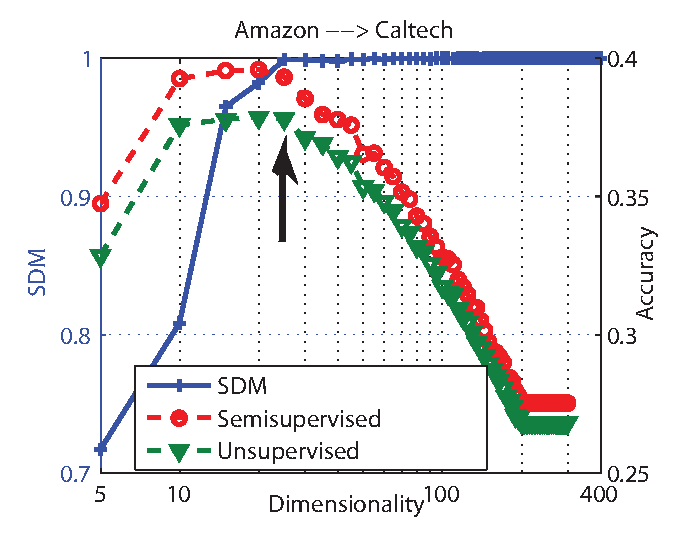
\includegraphics[width=0.45\columnwidth]{fig/fChoose_dim_amazon_caltech.eps} \quad 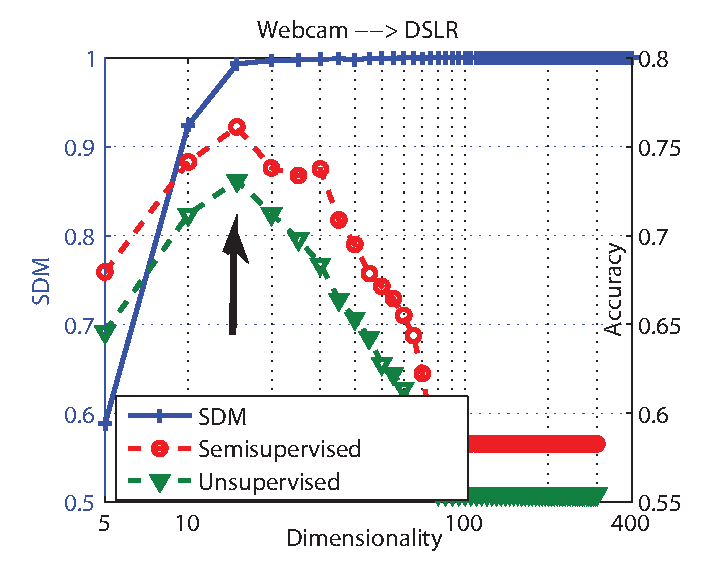
\includegraphics[width=0.45\columnwidth]{fig/fChoose_dim_webcam_dslr.eps} \\
  \caption{Selecting the optimal dimensionality $\cst{d}^*$ with SDM (sec. \ref{sDim}); selected $\cst{d}^*$ (where the arrows point to) leads to the best adaptation performance. (Best viewed in color)}\label{fig-choose-dim}
\end{figure*}


Being able to choose the optimal dimensionality for the subspaces is an important property of our methods. Fig.~\ref{fig-choose-dim} shows that the subspace disagreement measure (SDM) described in section~\ref{sDim} correlates well with  recognition accuracies on the target domains. In the plots, the horizontal axis is the proposed dimensionality (in $\log$ scale) and the right vertical axis reports accuracies on both unsupervised domain adaptation and semi-supervised domain adaptation.  The left vertical axis reports the values of SDM.

The plots reveal two conflicting forces at play. As the dimensionality increases, SDM---as a proxy to difference in geometric structures---quickly rises and eventually reaches its maximum value of 1. Beyond that point, adaptation becomes difficult as the subspaces have orthogonal directions.

However, before the maximum value is reached, the geometric difference is countered by the increase in variances --- a small dimensionality would capture very little variances in the source domain data and would result in poor accuracies on both  domains. The tradeoff occurs at where the geometric difference is just being maximized, justifying our dimensionality selection criterion in eq.~(\ref{eDim2}).
}

\subsection{Adaptation via the landmark based approach}
\label{sLandmarkResults}

Next we test our landmark adaptation approach.  For the hyper-parameters, we set the threshold of $\beta_m$ in eq.~(\ref{eSelected}) to be a small number ($10^{-8}$--$10^{-10}$) due to floating point arithmetics. {The RBF kernel bandwidths in eq.~(\ref{eRBF}) are $\sigma_q = 2^q\sigma_0$ with $q\in\{-6, -5, \cdots, 5, 6\}$, where $\sigma_0$ is the median of pairwise distances between all training instances. This ensures} we select at least one instance per category and we do not select all instances from the source domains as landmarks.  The SVM tradeoff parameters are tuned on the validation data, cf. section~\ref{sMKL}.  %In general, our experimental results are robust as long as we follow these mild guidelines.

{\bf Recognition accuracies.} Table~\ref{tResults} reports object recognition accuracies on the \emph{target} under nine pairs of source and target domains --- we did not use DSLR as the source domain  as it is too small to select landmarks. We contrast the proposed approach (\ours) to the methods of transfer component analysis (\textsc{tca}) \cite{tca}, geodesic flow sampling (\textsc{gfs}) \cite{gopalan2011domain}, our GFK approaches respectively with 1-NN and linear SVM (\textsc{gfk + 1nn} and \textsc{gfk + sum}), structural correspondence learning (\textsc{scl}) \cite{BlitzerEMNLP06Domain}, kernel mean matching (\textsc{kmm}) \cite{huang07correcting}, and a metric learning method (\textsc{metric}) \cite{saenko2010adapting}. Note \textsc{metric} is for \emph{semi-supervised} domain adaptation, so we reveal the labels of one instance per category from the target domains. We also report the baseline results of \textsc{no adapt} described in section~\ref{sGFKResults}.%, where we use source-only data and the original features to train classifiers.

\begin{table*}[t]
\centering
\caption{Recognition accuracies on 9 pairs of unsupervised domain adaptation via the landmark based approach. (C: Caltech, A: Amazon,
W: Webcam, and D: DSLR)  \eat{The proposed method (\textsc{gfk+landmark}) performs the best on 8 out of 9 pairs, among all unsupervised methods.}} \label{tResults}
\centering
\vskip 0.3em
\begin{tabular}{lccccccccc}
\toprule
\% & A$\rightarrow$C & A$\rightarrow$D & A$\rightarrow$W & C$\rightarrow$A & C$\rightarrow$D & C$\rightarrow$W & W$\rightarrow$A & W$\rightarrow$C & W$\rightarrow$D\tabularnewline
\midrule
\OrigFeat & 41.7 & 41.4 & 34.2 & 51.8 & 54.1 & 46.8 & 31.1 & 31.5 & 70.7 \\ \midrule
\textsc{tca}~\cite{tca} & 35.0 & 36.3 & 27.8 & 41.4 & 45.2 & 32.5 & 24.2 & 22.5 & 80.2 \\
\textsc{gfs}~\cite{gopalan2011domain} &  39.2  & 36.3  & 33.6  & 43.6 & 40.8 & 36.3 & 33.5 & 30.9 & 75.7 \tabularnewline
\textsc{gfk+1NN} (ours) & 42.2  & 42.7 & 40.7 & 44.5 & 43.3 & 44.7 & 31.8 & 30.8 & 75.6 \tabularnewline
\textsc{gfk+svm} (ours) & 38.8 & 43.3 & 37.3 & 50.2 & 40.1 & 45.1 & 39.1 & 34.5 & 67.5\tabularnewline
\textsc{scl}~\cite{BlitzerEMNLP06Domain} & 42.3 & 36.9 & 34.9 & 49.3 & 42.0 & 39.3 & 34.7 & 32.5 & \textbf{\textcolor{red}{83.4}} \tabularnewline
\textsc{kmm}~\cite{huang07correcting} & 42.2 & 42.7 & 42.4 & 48.3 & 53.5 & 45.8 & 31.9 & 29.0 & 72.0\tabularnewline
\textsc{metric}~\cite{saenko2010adapting} & 42.4 & 42.9 & {\color{red}\textbf{49.8}} & 46.6 & 47.6 & 42.8 & 38.6 & 33.0 & \textbf{\color{red}87.1} \tabularnewline \midrule
\textsc{gfk + landmark}~(ours) & \textbf{\textcolor{red}{45.5}} & \textbf{\textcolor{red}{47.1}} & \textbf{\textcolor{red}{46.1}} & \textbf{\textcolor{red}{56.7}} & \textbf{\textcolor{red}{57.3}} & \textbf{\textcolor{red}{49.5}} & \textbf{\textcolor{red}{40.2}} & \textbf{\textcolor{red}{35.4}} & 75.2\tabularnewline \bottomrule
\end{tabular}
\end{table*}



Our approach \ours\ clearly performs the best on almost all pairs, even when compared to the \textsc{metric} method which has access to labels from the target. The only significant exception is on the pair $\webcam\rightarrow\dslr$. Error analysis reveals that the two domains are very similar, containing images of the same object instances with different imaging resolutions. As such, many data points in \webcam\ are selected as landmarks, leaving very few instances for model selection. %Addressing this issue is left for future work.

{\bf Detailed analysis on landmarks.} Next, we further examine the utility of landmarks in domain adaptation to better understand why they are working as well as they do. We first study whether \emph{automatically selected} landmarks coincide with our modeling intuition, i.e., that they look like samples from the target domain.




\begin{figure*}[t]
  \centering
  \footnotesize
  \begin{tabular}{c|c|c}
    Examples  from {\webcam} (target)  &  Landmarks at scale $\sigma=2^6\sigma_0$   & Landmarks  at scale $\sigma=2^3\sigma_0$\\
    \includegraphics[width=0.32\textwidth]{fig/headphone_target.eps} &  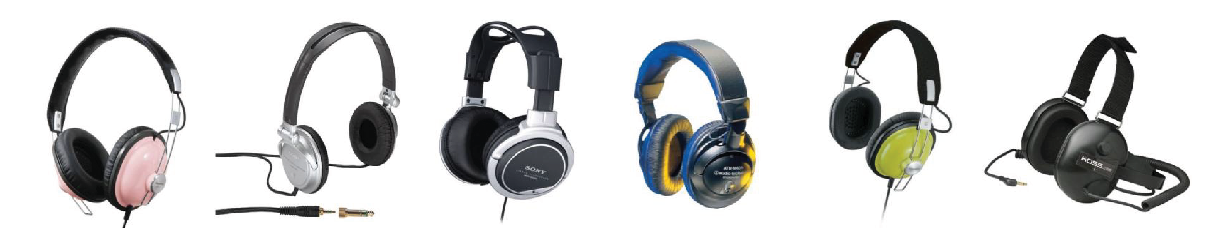
\includegraphics[width=0.32\textwidth]{fig/headphone_s6.eps}  & 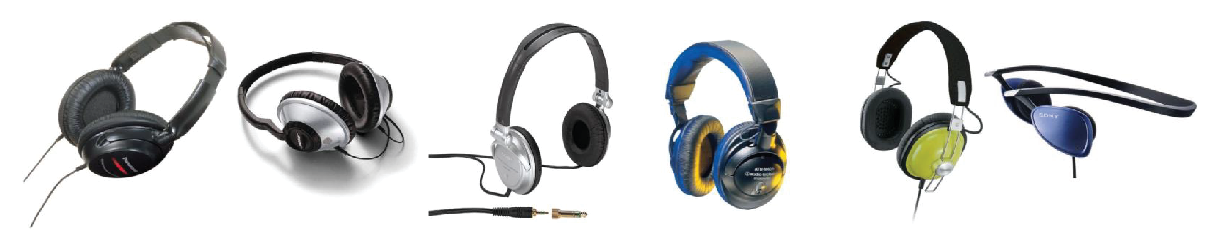
\includegraphics[width=0.32\textwidth]{fig/headphone_s3.eps}\\ 
    \includegraphics[width=0.32\textwidth]{fig/mug_target.eps} &  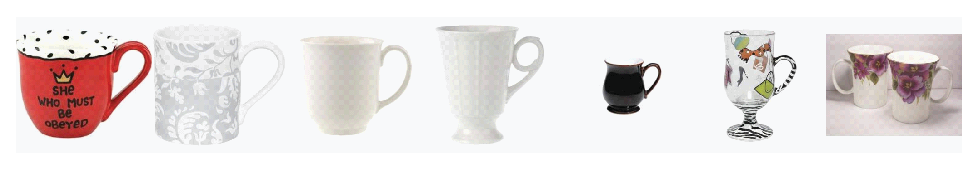
\includegraphics[width=0.32\textwidth]{fig/mug_s6.eps}  & 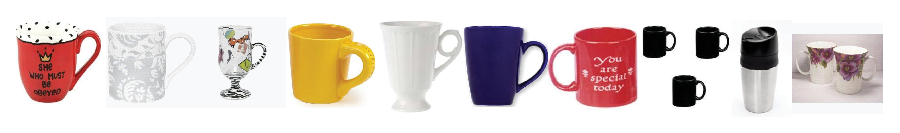
\includegraphics[width=0.32\textwidth]{fig/mug_s3.eps} \\
    Landmarks  at scale $\sigma=2^0\sigma_0$ & Landmarks  at scale $\sigma=2^{-3}\sigma_0$ & Examples of non-landmarks \\
    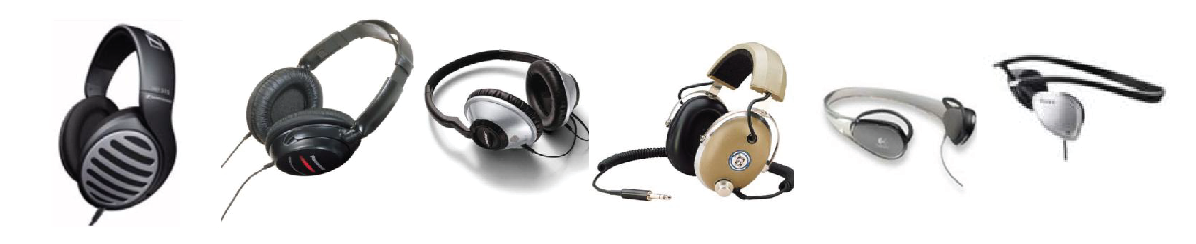
\includegraphics[width=0.32\textwidth]{fig/headphone_s0.eps} &  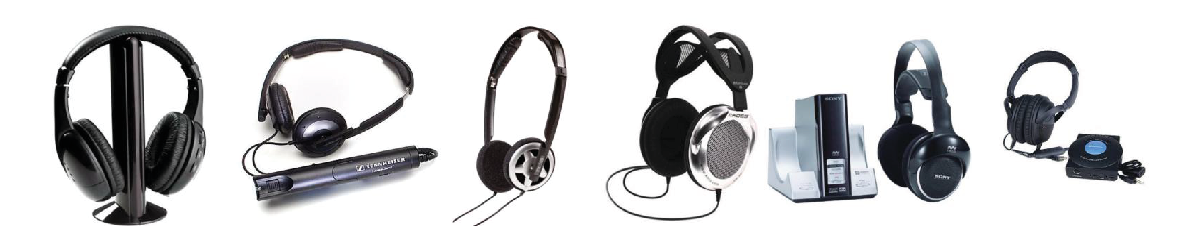
\includegraphics[width=0.32\textwidth]{fig/headphone_s_3.eps}  & 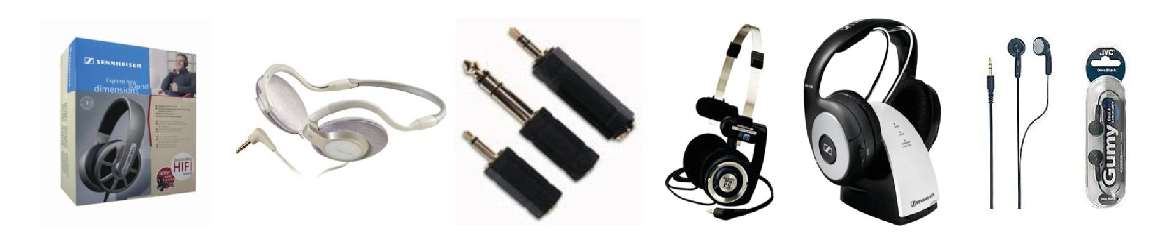
\includegraphics[width=0.32\textwidth]{fig/non_landmark.eps}\\ 
    \includegraphics[width=0.32\textwidth]{fig/mug_s0.eps} &  \includegraphics[width=0.32\textwidth]{fig/mug_s_3.eps}  & 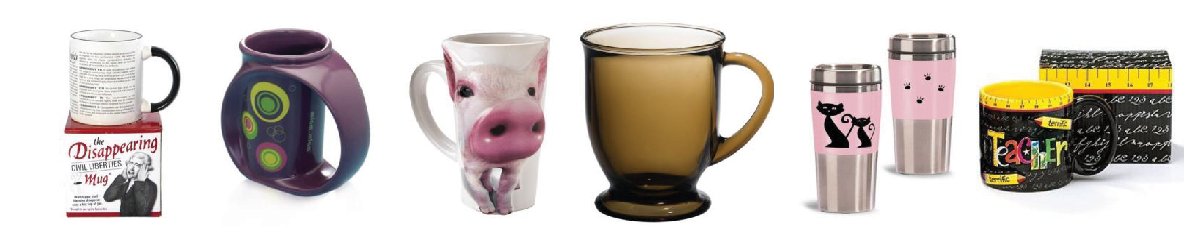
\includegraphics[width=0.32\textwidth]{fig/non_landmark_more.eps}\\
    %\textsc{mug}  from \webcam  &  Landmarks at scale $\sigma=2^6\sigma_0$   & Landmarks  at scale $\sigma=2^3\sigma_0$\\
    %\includegraphics[scale=0.2]{fig/mug_target.eps} &  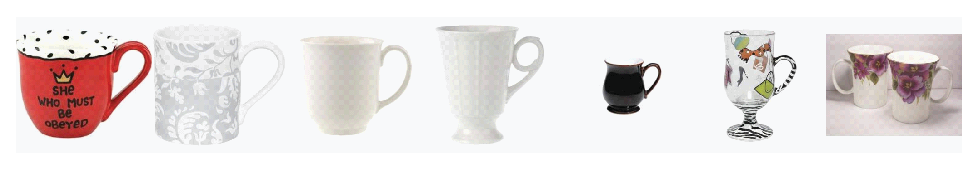
\includegraphics[scale=0.2]{fig/mug_s6.eps}  & 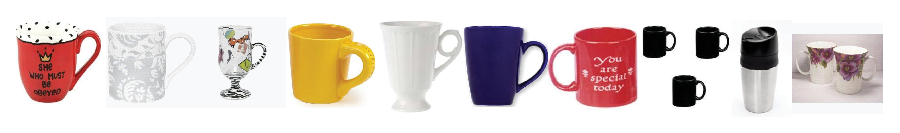
\includegraphics[scale=0.2]{fig/mug_s3.eps}\\ \hline
    %Landmarks  at scale $\sigma=2^0\sigma_0$ & Landmarks  at scale $\sigma=2^{-3}\sigma_0$ & Examples of non-landmarks \\
    %\includegraphics[scale=0.24]{fig/mug_s0.eps} &  \includegraphics[scale=0.24]{fig/mug_s_3.eps}  & 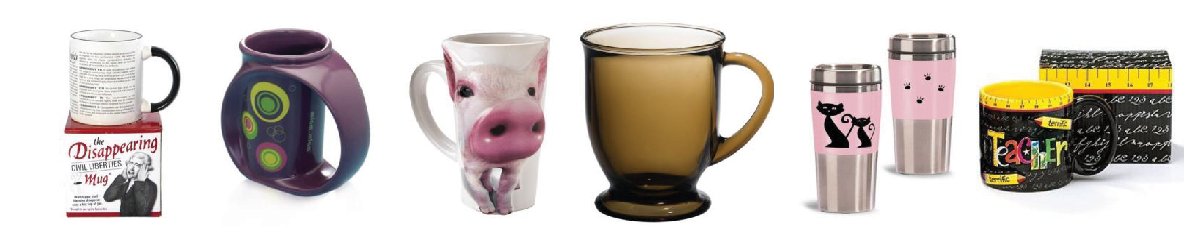
\includegraphics[scale=0.24]{fig/non_landmark_more.eps}\\ \hline
   \end{tabular}
    \caption{Landmarks selected from the source domain \amazon\ for the target domain \webcam, as well as non-landmarks (best viewed in color). As the scale decreases, images with greater variance in appearance are selected, as expected (cf.\ {\bf Multiscale analysis} in section~\ref{sFindLandmark}).}\label{fLandmark}
   \end{figure*}




Fig.~\ref{fLandmark} confirms our intuition. It displays several landmarks selected from the source domain \amazon\ when the target domain is \webcam. The top-left panel shows representative images from the \textsc{headphone} and \textsc{mug} categories from {\webcam}, and the remaining panels display images from \amazon, including both landmarks and those which are not. When the scale $\sigma$ is large, the selected landmarks are very similar in visual appearance to the images of the target. As the scale decreases, landmarks with greater variance show up. This is particularly pronounced at $2^{-3}\sigma_0$. Nonetheless, they still look far more likely to be from the target {\webcam} domain than non-landmark images (see the bottom-right panel) --- the non-landmarks for the \textsc{headphone} category contain images such as earphones and packaging boxes. Similarly, non-landmarks for the \textsc{mug} category are more unusually shaped ones.




\begin{table*}[t]
\centering
\caption{Contrasting  landmark selection algorithm to several variants. (C: Caltech, A: Amazon,
W: Webcam, and D: DSLR) }%C: \caltech, A: \amazon, W: \webcam, D: \dslr.  The proposed method (\textsc{landmark}) performs the best on almost all pairs.}
\label{tVariants}
\begin{tabular}{lccccccccc}
\toprule
\% & A$\rightarrow$C & A$\rightarrow$D & A$\rightarrow$W & C$\rightarrow$A & C$\rightarrow$D & C$\rightarrow$W & W$\rightarrow$A & W$\rightarrow$C & W$\rightarrow$D\tabularnewline
\midrule
\textsc{gfk + landmark}~(ours) & \textbf{\textcolor{red}{45.5}} &  \textcolor{black}{47.1} & 46.1 & \textbf{\textcolor{red}{56.7}} & \textbf{\textcolor{red}{57.3}} & 49.5 & \textbf{\textcolor{red}{40.2}} & \textbf{\textcolor{red}{35.4}} & \textbf{\textcolor{red}{75.2}}\tabularnewline \midrule
\textsc{Rand. Sel.} & 44.5 & 44.5  & 41.9 & 53.8  & 49.9  & 49.5  & 39.8 & 34.1 & 74.2\tabularnewline 
\textsc{Swap} & 41.3 & \textbf{\textcolor{red}{47.8}} & 37.6 & 46.2 & 42.0 & 46.1 & 38.2 & 32.2 & 70.1\tabularnewline 
\textsc{unbalanced} & 37.0 & 36.9 & 38.3 & 55.3 & 49.0 & \textbf{\textcolor{red}{50.1}} & 39.4 & 34.9 & 73.9\tabularnewline
\textsc{euc + landmark} & 44.5 & 44.0 & 41.0 & 50.2 & 40.1 & 45.1 & 39.1 & 34.5 & 67.5\tabularnewline \bottomrule
\end{tabular}
\end{table*}






In Table~\ref{tVariants}, we contrast our method to some of its variants, illustrating quantitatively the novelty and significance of using landmarks to facilitate adaptation. First, we study the adverse effect of selecting incorrect images as landmarks.  The row of \textsc{rand.~sel.}\  displays results of randomly selecting landmarks, as opposed to using the algorithm proposed in section~\ref{sLandmark}. (The number of random landmarks is the average number of ``true'' landmarks chosen in \ours.)
The averaged accuracies over 10 rounds are reported.   \textsc{gfk+landmark} outperforms the random strategy, often by a significant margin, validating the automatic selection algorithm.

The \textsc{swap} row in Table~\ref{tVariants} gives yet another strong indication of how landmarks could be viewed as  samples from the target. Recall that landmarks are used as \emph{training} data in the final stage of our learning algorithm (cf. section~\ref{sMKL}), while non-landmarks in the source are used for model selection. This setup follows the intuition that as landmarks are mostly similar to the target, they are a better proxy than non-landmarks for optimizing discriminative loss for the target. When we swap the setup, the accuracies drop significantly, except on the pair $A\rightarrow D$ (compare the rows \textsc{swap} and \textsc{gfk+landmark}).  This once again establishes the unique and extremely valuable role of the landmarks automatically selected by our algorithm.

We also study the class balancing constraint in eq.~(\ref{eBalance}), which enforces that the selected landmarks obey the class prior distribution. Without it, some classes dominate and  result in poor classification results. This is clearly evidenced in the row of  \textsc{unbalanced} where accuracies drop significantly after we remove the constraint.


\begin{SCfigure}
  % Requires \usepackage{graphicx}
  \centering
    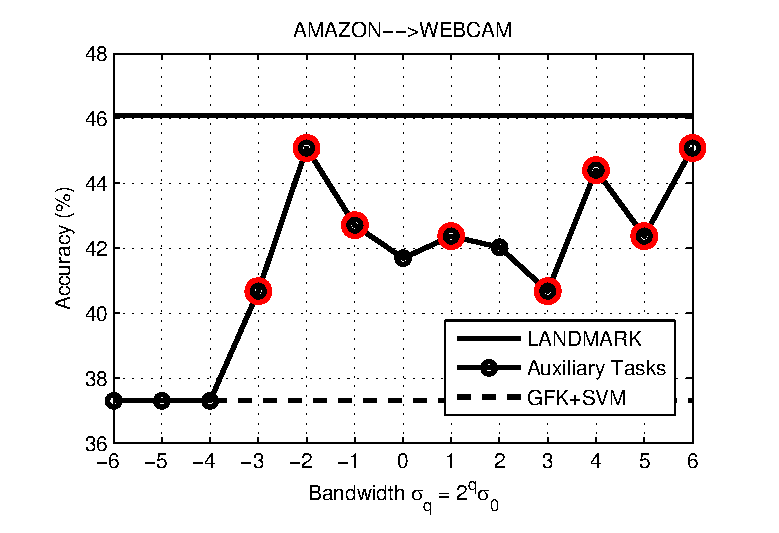
\includegraphics[width=0.5\columnwidth]{fig/AtoW_diff_sigma.eps}
  \caption{Performance of individual auxiliary tasks. Each circle point on the curves shows recognition accuracy on the original target domain $\tgt$, by using the kernel computed from the auxiliary task. All the circle points are above \textsc{gfk + sum} except when the scale is very small and results in that almost all source domain data are selected as landmarks. The red circles denote the auxiliary tasks whose kernels contribute to the final kernel $\mat{F}$ in eq.~(\ref{eMKL}) after  discriminative learning. }\label{fAuxiliary}
\end{SCfigure}



Finally, we study the effect of using GFK  to measure distribution similarity, as in eq.~(\ref{eRBF}). The row of \textsc{euc. + landmark} reports the results of using the conventional Euclidean distance, illustrating the striking  benefit of using GFK (in the row of \textsc{gfk+landmark}).
While using nonparametric two-sample tests to measure distribution similarity has been previously used for domain adaptation (e.g., kernel mean matching, cf. the row of \textsc{kmm} in Table~\ref{tResults}), selecting a proper kernel has received little attention, despite its vital importance. Our comparison to \textsc{euc. sel.} indicates that
measuring distribution similarity \emph{across} domains is greatly enhanced with a kernel revealing domain-invariant features.

{\bf Value of auxiliary tasks and multi-scale analysis.} The auxiliary tasks are domain adaptation problems over the auxiliary tasks --- the new pairs of source and target domains $\src^q \rightarrow \tgt^q$, cf. section~\ref{sAuxiliary}. As indicated by Theorem~1, by incorporating landmarks in the augmented target domain, the auxiliary adaptation problems become easier to solve. Fig.~\ref{fAuxiliary} provides strong empirical evidence supporting the theorem.  In the figure, we show the object recognition accuracies on the original target domain as a result of solving those auxiliary tasks individually.  Specifically, for each scale $\sigma_q$, we use the method of GFK to compute $\mat{G}_q$ for the pair $\src^q \rightarrow \tgt^q$ to extract invariant features and then train a SVM classifier using the landmarks (and their labels).  We contrast to \textsc{gfk+svm} reported in Table~\ref{tResults}, where the only difference from the experiments here is to solve the original adaptation problem. Clearly, the auxiliary tasks are easier to solve, resulting in more effective adaptations such that the accuracies on the target domains are in general much better than \textsc{gfk+svm}. This asserts firmly that landmarks bridge between the source and the target, and thus are an important adaptation mechanism to exploit.

In  Fig.~\ref{fAuxiliary}, we also contrast results of individual tasks to the proposed method \ours\ where the solutions of multiple auxiliary tasks are \emph{combined} discriminatively. Combination clearly improves on individual tasks, verifying the effectiveness of combination and our hypothesis that the data is modeled better at multiple scales. We mark in red color those individual tasks whose kernels have contributed to the final solution in eq.~(\ref{eMKL}). 




\eat{

\subsection{Which source domain should we use to adapt? } \label{sROD}
Imagine we need to build a classifier for a target domain for object recognition. We have several datasets, Caltech-101, PASCAL VOC, and ImageNet to choose from as the source domain. Without actually running our domain adaptation algorithms and building classifiers, is it possible to determine which dataset(s) would give us the best performance on the target domain?  This question is of practical importance: it is much more cost-effective to be able to select  one (or a limited few) that are likely to adapt well to the target domain, instead of trying each one of them.

To answer this question, we introduce a Rank of Domain (ROD) metric that integrates two sets of information: geometrically, the alignment between subspaces, and  statistically, KL divergences between data distributions once  they are projected into the subspaces.

\paragraph{Rank of Domain (ROD) metric} We sketch the main idea in the following; the detailed derivation is
described in the Appendix~\ref{sec-ROD}. Given a pair of domains, computing ROD
involves three steps: i) determine the optimal dimensionality
$\cst{d}^*$ for the subspaces (as in section~\ref{sDim}); ii) at
each dimension $i\le\cst{d}^*$,  approximate the data distributions of
the two domains with two one-dimensional Gaussians and then compute
the symmetrized KL divergences between them; iii) compute the KL-divergence
weighted average of principal angles, namely,
\begin{equation}
\mathcal{R}(\mathcal{S},\mathcal{T}) = \frac{1}{\cst{d}^*}\sum_{i}^{{\cst{d}^*}}\theta_i \left[KL(\mathcal{S}_i \| \mathcal{T}_i) + KL(\mathcal{T}_i\|\mathcal{S}_i)\right].
\end{equation}
$\mathcal{S}_i$ and $\mathcal{T}_i$ are the two above-mentioned Gaussian distributions; they are estimated from data projected  onto the principal vectors (associated with the $i$-th principal angle).  Note that we use only the first $\cst{d}^*$ directions. Beyond that, the two subspaces of the source and target domains start to have orthogonal directions, on which the two domains would have very different geometric and statistical properties. As such, the source classifier is unlikely to be adapted successfully to the target.

A pair of domains with smaller values of $\mathcal{R}(\mathcal{S},\mathcal{T})$ are more likely to adapt well:  the two domains are both geometrically well-aligned (small principal angles) and similarly distributed (small KL divergences).  Empirically, when we use the metric to rank various datasets as source domains, we find the ranking correlates well with their relative performance improvements on the target domain.

\begin{table}
  \centering
  \caption{ROD values between 4 domains. Lower values signify stronger adaptability of the corresponding source domain.}\label{tROD}
  \begin{tabular}{|c|c|c|c|c|}
    \hline
     $\rightarrow$ & \caltech & \amazon & \dslr & \webcam \\ \hline
    \caltech & 0 & \textbf{0.003} & 0.21 & 0.09 \\ \hline
    \amazon & \textbf{0.003} & 0 & 0.26 & 0.05 \\ \hline
    \dslr & 0.21 & 0.26 & 0 & \textbf{0.03} \\ \hline
    \webcam & 0.09 & 0.05 & \textbf{0.03} & 0 \\
    \hline
    \end{tabular}
   \end{table}

}

\eat{
\paragraph{Empirical verification of ROD}  Now we examine whether  the ROD metric correlates with our empirical findings.  We compute ROD using PCA subspaces and report the values among the four domains in  Table \ref{tROD}. In general, ROD correlates well with recognition accuracies on the target domains and can reliably identify the best source domains to adapt. For example, when  \caltech\ is the target domain (the first column),  \amazon\ has the smallest value and \amazon\ indeed leads to  better classification accuracies on \caltech\ than \dslr\ or \webcam. We find that the ROD metric also corroborates strongly with recognition accuracies for \emph{semi-supervised} domain adaptation, cf. Table~\ref{tSemi-Caltech} in the Appendix. This further supports the value of the ROD metric as a barometer indicating whether two datasets are intrinsically similar, in both geometrical and statistical properties.

If we group \caltech\ and \amazon\ into a meta-category ``Online'' and \dslr\ and \webcam\ into another meta-category ``Office'',  the distributions of ROD values with respect to the categories suggest that the domains with the same meta-category have stronger similarity than domain pairs crossing categories (such as \caltech\ and \dslr).
Thus ROD can also be used as a measure to partition datasets into clusters, where datasets in the same cluster share latent properties that might be of surprise to their users --- the presence of such properties is probably not by design.


\subsection{Ease of adaptation: a new perspective on datasets?}
\label{sAdaptability}


\begin{table*}[t]
  \centering
  \caption{Cross-dataset generalization with and without domain adaptation among domains with high and low ``market values'' \cite{TorralbaCVPR11Unbiased} } \label{tRevisit}
  \begin{tabular}{|c|ccc|c|c||ccc|c|c|c|}
    \hline
    \% & \multicolumn{5}{|c||}{No domain adaptation}  & \multicolumn{6}{|c|}{Using domain adaptation} \\ \hline
    $\rightarrow$ & P & I & C101 &  Mean Targets & Drop$_1$ & P & I & C101 & Mean Targets  & Drop$_2$ & Improvement \\ \hline \hline
    PASCAL & \textbf{37.9} & 38.5 & 34.3 &  36.4 & \textbf{4\%}         & -- & 43.6 & 39.8 & 41.7 & \textbf{-10\%} &\textbf{14\%} \\ \hline
    ImageNet & 38.0 & \textbf{47.9} & 40.0 & 39.0 & \textbf{19\%}          & 42.9 & -- & 49.1 & 46.0 & \textbf{4\%} &\textbf{18\%} \\ \hline
    Caltech101 & 31.9 & 38.6 & \textbf{66.6} &  35.3 & \textbf{47\%}          & 34.1 & 37.4 & -- & 35.8 & \textbf{46\%} &\textbf{1\%} \\
    \hline
  \end{tabular}
 \end{table*}


\citet{TorralbaCVPR11Unbiased} study the sources of dataset bias and the problem of cross-dataset generalization in several popular ones for object recognition \cite{TorralbaCVPR11Unbiased}. To quantify the quality of each dataset, they devise a ``market value'' metric. Datasets with higher values are more diverse, and therefore are likely to reflect better the richness of real-world objects. In particular, they point out that PASCAL VOC 2007 and ImageNet have high values.  However, we hypothesize that the market values could in some cases be overly pessimistic, since in their study no attempts were made to explicitly account for domain shifts between datasets.

Thus, building on their findings, we turn the tables around and investigate: \emph{how valuable are these  datasets  in improving a target domain's performance?}

Table \ref{tRevisit} summarizes our results on a subset of datasets used in \cite{TorralbaCVPR11Unbiased}; PASCAL VOC 2007 \cite{pascal-voc-2007}, ImageNet \cite{DengCVPR09Imagenet}, and Caltech-101 \cite{fei2007learning}.  The recognition tasks are to recognize the category \emph{person} and \emph{car}.
The cross-dataset generalization results are shown on the left side of the table, without using adaptation techniques (as in \cite{TorralbaCVPR11Unbiased});  and the adaptation results using our kernel-based method are on the right side of the table.

The rows are the source domain datasets and the columns are the target domains. The ``Drop'' columns report the percentages of drop in recognition accuracies between the source and the averaged accuracy on target domains, ie, the ``Mean Targets'' columns.  The rightmost ``Improvement'' column is  the percentage of improvement on target domains due to the use of domain adaptation. Clearly, domain adaptation noticeably improves recognition accuracies on the target domains. Caltech-101 is the exception where  the improvement is marginal (47\% vs.~46\%). This corroborates the low ``market value'' assigned to this dataset in \cite{TorralbaCVPR11Unbiased}.

PASCAL VOC 2007 has the smallest drop without domain adaptation so it would appear to be a better dataset than the other two.
Once we have applied domain adaptation, we observe a negative drop --- ie, the performance on the target domains is better than on the source domain itself! However, its improvement is not as high as ImageNet's.

Our conjecture is that  the data in PASCAL VOC 2007 can be partitioned into two parts: one part is especially ``hard'' to be adapted to other domains and the other part is relatively ``easy''. The reverse of the performance drop suggests that the ``easy'' portion can be harvested by domain adaptation techniques. However, the benefit is limited due to the ``hard'' part. On the other end, for ImageNet, a larger portion of its data is perhaps amenable to adaptation. Hence, it attains a bigger improvement after adaptation.

In short, while PASCAL VOC 2007 and ImageNet are assigned the same ``market value'' in \cite{TorralbaCVPR11Unbiased}, their usefulness to building object recognition systems that can be applied to  other domains needs to be carefully examined in the context of adaptation. It might be beneficial to incorporate the notion of ``ease of adaptability'' in the process of evaluating datasets --- a concept worth further exploring and refining.

}




%\section{Related Work}
\label{sRelated}

Domain adaptation has been extensively studied  in many areas, including in
statistics and machine learning \cite{shimodaira00shift,huang07correcting,bendavid07domain,pan2009survey},
speech and language
processing \cite{daume07easy,BlitzerEMNLP06Domain,LeggetterCSL95Maximum},
and more recently computer
vision \cite{bergamo09weak,gopalan2011domain,saenko2010adapting,kulisyou}.

Of particular relevance to our kernel methods  is the idea of learning feature representations that are domain-invariant, thus enabling transferring classifiers from the source domain to the target domain \cite{bendavid07domain,BlitzerEMNLP06Domain,BlitzerACL07domain,daume07easy,tca}.
The feature representation can be derived from using auxiliary tasks that predict ``pivot features''~\cite{ando05,BlitzerEMNLP06Domain}, augmenting the feature space~\cite{daume07easy,daume10co,li2012discriminative,gopalan2013learning}, co-training with multi-view representations~\cite{chen11cotrain}, or matching probabilistic distributions~\cite{tca}.
Those approaches are especially appealing to unsupervised domain adaptation as they  do not require labeled target data. %Other methods for unsupervised domain adaptation have been explored, for example, with transductive SVMs \cite{bergamo09weak} or iteratively relabeling (the target domain) \cite{bruzzone2010domain}.

Gopalan \emph{et al.}'s work is the closest to our GFK approach in spirit \cite{gopalan2011domain}. They have also explored the idea of using geodesic flows to derive intermediate subspaces that interpolate between the source and target domains. A crucial difference from ours is that they sample a \emph{finite} number of subspaces and stack these subspaces into a very high-dimensional projection matrix. As such, the dimension of their features needs to be reduced. This extra step, unfortunately, might introduce modeling errors and practical challenges. For instance, it is not clear how to choose the subspace sampling rate or the right feature dimension after reduction. %and whether the dimension reduction method used there necessarily helps classification.

In stark contrast, GFK is both conceptually and computationally simpler and eliminates the need to tune many hyper-parameters as by Gopalan \emph{et al.}'s approach. In particular, our kernel is in closed form, and computing it involves simple matrix algebra for example singular value decomposition. We have devised a fully automatic procedure, which is lacking in Gopalan \emph{et al.}'s work,  to choose the optimal dimensionality of the subspaces. {We also note that Zheng {\it et al.} proposed the same kernel, albeit independently and almost simultaneously~\cite{zheng2012grassmann}, though they did not offer an automatic procedure to determine the dimensions of the subspaces.}


While learning domain-invariant feature representations has been extensively studied in the literature, identifying and using instances that are distributed similarly to the target to bridge the two domains, as in our landmark-based approach,  has not been explored before.

The idea of auxiliary tasks was explored previously in \cite{BlitzerEMNLP06Domain} to identify invariant features. There, the tasks were to predict ``pivot features''. The derived features are PCA directions of those predictive models' parameters.  In our landmark-based approach,  however, the auxiliary tasks are new \emph{domain adaptation} tasks and the invariant features are learned \emph{discriminatively}. 

The procedure of moving labeled data between the source and the target domains in our landmark approach is similar in spirit to transductive style domain adaptation methods~\cite{bergamo09weak,bruzzone2010domain,chen11cotrain} where classifiers are iteratively retrained after labeled examples are moved.  Our approach has several crucial differences. First, we partition the source domain into two disjoint subsets, only once for each auxiliary task. We do not iteratively re-partition the data or iteratively re-train the classifiers.  Secondly, our primary goal is to learn useful features/kernels from each auxiliary task, while those methods  use the original features and aim to incrementally learn classifiers. Moreover, they depend very much on manually tuning several  parameters, which requires extensive computation of training and cross-validation.

Kernel mean matching has previously been used to \emph{weigh} samples from the source \cite{huang07correcting,tca,gretton09kmm} to correct the mismatch between domains. We \emph{select} samples as our landmarks. Those prior works typically do not yield sparse solutions (of the weights), and thus do not perform \emph{selection}.  Additionally, the inclusion of the balancing constraint in our formulation of eq.~(\ref{eSelected}) is crucial, as evidenced in our experimental studies (cf. Table~\ref{tResults} ). Without it, some classes could be underrepresented in selected landmarks, leading to poor performance.%%% due to unbalanced priors.

Broadly, our emphasis on learning kernels is relevant to the approaches of metric learning for domain adaptation, where the Mahalanobis metric  is a form of linear kernel functions~\cite{saenko2010adapting,kulisyou,shi2012}. Our GFK approach implicitly relies on the discriminative clustering assumption to reduce the discrepancy between how pairwise distances among data points are distributed in two domains. Such an assumption is explicitly exploited to derive an objective function to ensure adaptation~\cite{shi2012}. 

%The proposed method differentiates from those efforts by synthesizing auxiliary domain adaptation tasks that repartition data in the source and the target domains. This is different from using auxiliary classification tasks to model correlations between features \cite{BlitzerEMNLP06Domain}. Our approach is also different from  where the source and the target domains also change iteratively. In particular, our approach repartitions only once for each auxiliary task by pushing identified landmarks into the unlabeled target domain. Transuctive-style algorithms operate the opposite way, by revealing labels of unlabeled target data and making them part of the labeled set.  Finally, most of the previously mentioned work do not learn discriminatively to combine outputs of auxiliary tasks as we do.

%An important algorithmic property of our formulation differentiates our work from other existing works in applying MMD to \emph{weigh} samples from source domains \cite{huang07correcting,tca}. In particular, our formulation often leads to \textbf{sparse} solutions where some $\beta_m$ are zeroes. The nonzero $\beta_m$ correspond to landmarks.  Indeed, we recover the solution to the binary $\alpha_m$ by  finding the support of $\beta_m$, ie, $\alpha_m = \textsc{sign}(\beta_m)$. Due to differences in constraints and objective functions, other work do not aim to yield sparse solutions.
%Analysis with multiple scaling parameters has been previously studied, for example, in spectral clustering where Gaussian kernels have also been used to measure similarities between data \cite{zelnik2004self}. The motivation there is to choose a proper local scaling that is specific to each data point.  Our motivation is different: we compare two sets of data points and need to choose a proper ``global'' scaling so that points from two different domains could be identified as similar. %Nevertheless, it is interesting to notice that the hard problem of choosing the right scale can be attacked in the context of completely unsupervised clustering. In our case, however, we have labeled data to leverage. We describe our strategy after we explain how to setup supervised learning problems.




% !TEX root = da.tex
\section{Conclusion} \label{sConclusion}

Unsupervised domain adaptation is an important yet quite challenging problem. Our work has shown that it is very effective to address it by leveraging and modeling intrinsic structures such as subspaces and landmarks in the data.  We propose  kernel-based approaches for unsupervised domain adaptation. 
The key insight behind our approaches is to learn kernel functions that correspond to (implicitly defined) feature spaces that are robust to the mismatch between the source and the target domains. 

Our first approach, the geodesic flow kernel (GFK), exploits the low-dimensional subspace structures in the visual data and measures similarity between data points in a way that is insensitive to each domain's idiosyncrasies.  It is simple to implement, free of hyperparmeter tuning, and performs very well in benchmark tasks. Our second approach builds on the success of GFK and exploits the landmark structures between two domains. Essentially, the landmarks are data points from the source domain but also serve as a bridge to  the target domain. The landmarks enable analyzing distribution similarity on multiple scales, hypothesizing a basis for invariant features, and discriminatively learning features/kernels. On benchmark tasks for visual recognition, this approach consistently outperforms  others (including the approach of GFK), often by large margins.  Furthermore, we show that the landmark approach is strongest when using the GFK as its component kernel.

This chapter has just scratched the surface of the domain adaptation problem in visual recognition. While we have shown that learning kernels is powerful in discovering feature spaces where the two domains are similar, learning kernels is potentially useful for answering more challenging problems: what is a domain?  and how can we characterize the difference between domains? Our paper~\cite{our2013reshape} sheds some light on these questions.  We challenge the conventional wisdom and practice that equates a dataset to a domain. Instead, we argue that vision datasets are likely a m\'{e}lange of multiple latent and heterogeneous domains. We propose new learning algorithms that identify the latent domains in a vision dataset. We then show that using the resulting domains to adapt is more effective than using the original dataset. 


Overall, the kernel learning framework opens the door for future research towards domain adaptation. For instance, GFK is just one possibility of averaging inner products from multiple subspaces interpolating between the source and target domains. It would be interesting to explore other choices. The auxiliary tasks in the landmark-based approach can be regarded as multiple sources, and multiple-source domain adaptation algorithms could be explored~\cite{dam,dredze08multi} jointly with the landmarks.

{

%Our success there thus validates again the central thesis that inspires the landmark approach. Namely, not every data instance has the same adaptability, as they all could come from unknown distributions with different degrees of proximity to the target domain. Thus, to be effective in adaptation, it is desirable \emph{not} to treat the source domain as being monolithically homogeneous. %It would be interesting to explore how to use kernel learning  to identify feature spaces that maximally \emph{distinguish} domains. We leave that for future research.
}


%%%% For future work, we plan to exploit other structures for adaptation.





%%%%%%% ACKNOWLEDGEMENTS %%%%%%%%%%%%%
\begin{acknowledgement}
This work is partially supported by DARPA D11-AP00278 and NSF IIS-1065243 (B.~G.\ and F.~S.), and ONR ATL \#N00014-11-1-0105 (K.~G.). The Flickr images in Fig.~1 are under a CC Attribution 2.0 Generic license, courtesy of berzowska, IvanWalsh.com, warrantedarrest, HerryLawford, yuichi.sakuraba, zimaowuyu, GrahamAndDairne, Bernt Rostad, Keith Roper, flavorrelish, and deflam.
\end{acknowledgement}




%%%%%%% References %%%%%%%%%%%%%

\bibliographystyle{plain}
\bibliography{DomAd,extra}


\end{document}
